\documentclass[12pt]{amsart}
\usepackage[margin=1in]{geometry} 
\usepackage{amsmath,amsthm,amssymb,setspace, mathtools}
\usepackage{physics}
\usepackage{tikz, tikz-cd, tkz-fct}  
\usepackage{pgfplots}

\usepackage{color}   %May be necessary if you want to color links
\usepackage{hyperref}
\hypersetup{
	colorlinks=true, %set true if you want colored links
	linktoc=all,     %set to all if you want both sections and subsections linked
	linkcolor=black,  %choose some color if you want links to stand out
	urlcolor=cyan
}


\pgfplotsset{every axis/.append style={
		axis x line=middle,    % put the x axis in the middle
		axis y line=middle,    % put the y axis in the middle
		axis line style={<->,color=black}, % arrows on the axis
		xlabel={$x$},          % default put x on x-axis
		ylabel={$y$},          % default put y on y-axis
}}

%
%
%
\newif\ifhideproofs
%\hideproofstrue %uncomment to hide proofs
%
%
%
%
\ifhideproofs
\usepackage{environ}
\NewEnviron{hide}{}
\let\proof\hide
\let\endproof\endhide
\fi

\theoremstyle{definition}
\newtheorem{definition}{Definition}[subsection]
\newtheorem{defn}[definition]{Definition}
\newtheorem{note}[definition]{Note}
\newtheorem{thm}[definition]{Theorem}
\newtheorem{lem}[definition]{Lemma}
\newtheorem{prop}[definition]{Proposition}
\newtheorem{cor}[definition]{Corollary}
\newtheorem{conj}[definition]{Conjecture}
\newtheorem{ex}[definition]{Exercise}

\newcommand{\al}{\alpha}
\newcommand{\gam}{\gamma}
\newcommand{\Gam}{\Gamma}
\newcommand{\bet}{\beta} 
\newcommand{\del}{\delta} 
\newcommand{\Del}{\Delta}
\newcommand{\lam}{\lambda}  
\newcommand{\Lam}{\Lambda} 
\newcommand{\ep}{\epsilon}
\newcommand{\sig}{\sigma} 
\newcommand{\om}{\omega}
\newcommand{\Om}{\Omega}
\newcommand{\C}{\mathbb{C}}
\newcommand{\N}{\mathbb{N}}
\newcommand{\E}{\mathbb{E}}
\renewcommand{\H}{\mathbb{H}}
\newcommand{\Z}{\mathbb{Z}}
\newcommand{\R}{\mathbb{R}}
\newcommand{\T}{\mathbb{T}}
\newcommand{\Q}{\mathbb{Q}}
\renewcommand{\P}{\mathbb{P}}
\newcommand{\MA}{\mathcal{A}}
\newcommand{\MC}{\mathcal{C}}
\newcommand{\MB}{\mathcal{B}}
\newcommand{\MF}{\mathcal{F}}
\newcommand{\MG}{\mathcal{G}}
\newcommand{\ML}{\mathcal{L}}
\newcommand{\MN}{\mathcal{N}}
\newcommand{\MS}{\mathcal{S}}
\newcommand{\MP}{\mathcal{P}}
\newcommand{\ME}{\mathcal{E}}
\newcommand{\MT}{\mathcal{T}}
\newcommand{\MI}{\mathcal{I}}
\newcommand{\MJ}{\mathcal{J}}
\newcommand{\MM}{\mathcal{M}}
\newcommand{\MX}{\mathcal{X}}

\newcommand{\tMA}{\tilde{\MA}}
\newcommand{\tMB}{\tilde{\MB}}


\newcommand{\tU}{\tilde{U}}
\newcommand{\tV}{\tilde{V}}
\newcommand{\tphi}{\tilde{\phi}}
\newcommand{\tpsi}{\tilde{\psi}}
\newcommand{\tF}{\tilde{F}}


\newcommand{\Tn}[1]{T^{r_{#1}}_{s_{#1}}(V)}
\newcommand{\Tnp}{T^{r_1 + r_2}_{s_1 + s_2}(V)}


\newcommand{\p}{\partial}

\renewcommand{\r}{\rangle}
\renewcommand{\l}{\langle}

\newcommand{\RG}{[0,\infty]}
\newcommand{\Rg}{[0,\infty)}
\newcommand{\Ll}{L^1_{\text{loc}}(\R^n)}

\newcommand{\limfn}{\liminf \limits_{n \rightarrow \infty}}
\newcommand{\limpn}{\limsup \limits_{n \rightarrow \infty}}
\newcommand{\limn}{\lim \limits_{n \rightarrow \infty}}
\newcommand{\convt}[1]{\xrightarrow{\text{#1}}}
\newcommand{\conv}[1]{\xrightarrow{#1}} 
\newcommand{\seq}[2]{(#1_{#2})_{#2 \in \N}}



\newcommand{\lex}[1]{\label{ex:#1}}
\newcommand{\ld}[1]{\label{defn:#1}}
\newcommand{\rex}[1]{Exercise \ref{ex:#1}}
\newcommand{\rd}[1]{Definition \ref{defn:#1}}


\DeclareMathOperator{\supp}{supp}
\DeclareMathOperator{\sgn}{sgn}
\DeclareMathOperator{\spn}{span}
\DeclareMathOperator{\iso}{Iso}
\DeclareMathOperator{\id}{id}
\DeclareMathOperator{\Aut}{Aut}
\DeclareMathOperator{\Homeo}{Homeo}
\DeclareMathOperator{\Sym}{Sym}
\DeclareMathOperator{\cl}{cl}
\DeclareMathOperator{\Int}{Int}
\DeclareMathOperator{\bal}{bal}
\DeclareMathOperator{\cnv}{conv}
\DeclareMathOperator{\epi}{epi}



\begin{document}
	
	\title{Introduction to Differential Geometry}
	\author{Carson James}
	\maketitle
	
	\tableofcontents
	
	\section{Review of Fundamentals}

	\subsection{Set Theory}
	
	\begin{defn}
		Let $\{A_i\}_{i \in I}$ be a collection of sets. The \textbf{disjoint union of} $\{A_i\}_{i \in I}$, denoted $\coprod\limits_{i \in I} A_i$, is defined by $$\coprod_{i \in I}A_i = \bigcup_{i\in I} \{i\} \times A_i$$ 
		We define the \textbf{natural projection map}, denoted $\pi: \coprod\limits_{i \in I} A_i \rightarrow I$, by $\pi(i, a) = i$.
	\end{defn}

	\begin{defn}
		Let $E$ and $M$ be sets, $\pi:E \rightarrow B$ a surjection and $\sig: B \rightarrow E$. Then $\sig$ is said to be a section of $(E, M, \pi)$ if $\pi \circ \sig = \id_{M}$. 
	\end{defn}

	\begin{note}
		Let $\{A_i\}_{i \in I}$ be a collection of sets and $\sig: I \rightarrow \coprod\limits_{i \in I} A_i$. We will typically be interested in sections $\sig$ of $\bigg( \coprod\limits_{i \in I} A_i, I, \pi \bigg)$.
	\end{note}

	\begin{ex}
		Let $\{A_i\}_{i \in I}$ be a collection of sets and $\sig: I \rightarrow \coprod\limits_{i \in I} A_i$. Then $\sig$ is a section of $\coprod\limits_{i \in I} A_i$ iff for each $i \in I$, $\sig(i) \in A_i$
	\end{ex}
	
	\begin{proof}
		Clear.
	\end{proof}
	
	\subsection{Smooth Maps}
	
	\begin{defn} \ld{21001}
		Let $n \geq 1$. For $i = 1, \cdots, n$, define $x^i: \R^n \rightarrow \R$ by $x^i(a^1, \cdots, a^n) = a^i$. The functions $(x^i)_{i=1}^n$ are called the \textbf{standard coordinate functions on $\R^n$}. 
	\end{defn}
	
	\begin{defn} \ld{21002}
		Let $U \subset \R^n$ be open, $f: U \rightarrow \R$ and $a \in U$. Then $f$ is said to be \textbf{differentiable with respect to $x^i$ at $a$} if $$\lim\limits_{h \rightarrow 0} \frac{f(a + he^i) - f(a)}{h}$$ exists. If $f$ is differentiable with respect to $x^i$ at $a$, we define the \textbf{partial derivative of $f$ with respect to $x^i$ at $a$}, denoted $$\frac{\partial f}{\partial x^i} (a) \text{ or } \eval{\pdv{x^i}}_{a} f $$ to be the limit above.
		
	\end{defn}
		
	\begin{defn} \ld{21003}
		Let $U \subset \R^n$ be open and $f: U \rightarrow \R$. Then $f$ is said to be \textbf{differentiable with respect to $x^i$} if for each $a \in U$, $f$ is differentiable with respect to $x^i$ at $a$.
	\end{defn}

	\begin{ex}\lex{21004}
		Let $U \subset \R^n$ be open, $f: U \rightarrow \R$ and $a \in U$. Suppose that $\frac{\partial ^2 f}{\partial x^i x^j}$ and $\frac{\partial ^2 f}{\partial x^j x^i}$ exist and are continuous at $a$. Then $$\frac{\partial ^2 f}{\partial x^i x^j} (a) = \frac{\partial ^2 f}{\partial x^j x^i} (a)$$
	\end{ex}

	\begin{proof}
		
	\end{proof}

	\begin{defn} \ld{21004}
		Let $U \subset \R^n$ be open and $f: U \rightarrow \R$. Then $f$ is said to be \textbf{smooth} if for each $i_1, \cdots, i_k \in \{1, \cdots, n\}$, $\frac{\partial^k f}{\partial i_1 \cdots i_k}$ exists and is continuous on $U$.
	\end{defn}

	\begin{defn} \ld{21005}
		Let $U \subset \R^n$, $f: U \rightarrow \R$. Then $f$ is said to be \textbf{smooth} if there exists $U' 
		\subset \R^n$ and $f':U' \rightarrow \R$ such that $U \subset U'$, $U'$ is open, $f'|_U = f$ and $f'$ is smooth. The set of smooth functions on $U$ is denoted $C^{\infty}(U)$.
	\end{defn}

%	\begin{defn} 
%		Let $U \subset \R^n$ and $p \in U$. Then $U$ is said to be \textbf{star-shaped} if for each $q \in U$, $\{p + t(q-p): 0 \leq t \leq 1\} \subset U$.
%	\end{defn}

	\begin{thm} \textbf{Taylor's Theorem:}\\ 
		Let $U \subset \R^n$ be open and convex, $p \in U$, $f \in C^{\infty}(U)$ and $T \in \N$. Then there exist $(g_{\al})_{|\al| = T+1} \subset C^{\infty}(U)$ such that for each $x \in U$, 
		$$f(x) = \sum_{k=0}^{T} \bigg[\sum_{|\al| = k}(x - p)^{\al} \p^{\al} f (p) \bigg] + \sum_{|\al| = T+1}(x - p)^{\al} g_{\al}(x)$$ and for each $|\al|= T+1$, $$g_{\al}(p) = \frac{1}{(T+1)!}\p^{\al} f(p)$$
	\end{thm}
	
	\begin{proof}
	See analysis notes
	\end{proof}

%	\begin{proof}
%		Let $x \in U$. Since $U$ is star-shaped with respect to $p$, $\{p + t(x-p): 0 \leq t \leq 1\} \subset U$. By the chain rule, 
%		$${\dv{t}} \bigg[ f(p+t(x-p)) \bigg] = \sum_{i=1}^n {\pdv{f}{x^i}}(p+t(x-p)) (x^i - p^i)$$
%		Integrating both sides with respect to $t$ from $0$ to $1$, we obtain
%		$$f(x) - f(p) = \sum_{i=1}^n (x^i - p^i) \int_{0}^{1}  {\pdv{f}{x^i}}(p+t(x-p)) dt $$
%		For $i \in \{1, \cdots, n\}$, define $g_i \in C^{\infty}(U)$ by $$g_i(x) = \int_{0}^{1}  {\pdv{f}{x^i}}(p+t(x-p)) dt$$
%		Then for each $i \in \{1, \cdots, n\}$, $$g_i(p) = {\pdv{f}{x^i}}(p))$$
%	\end{proof}

	\begin{defn}
	Let $U \subset \R^n$ and $F: U \rightarrow \R^m$. Let $x^1, \cdots, x^n$ be the standard coordinate functions on $\R^n$ and $y_1, \cdots, y_m$ be the standard coordinate functions on $\R^m$. For $i \in \{1, \cdots, m\}$, we define the \textbf{$i$th component of $F$}, denoted $F^i: U \rightarrow \R$, by $$F^i = y^i \circ F$$ 
	Thus $F = (F_1, \cdots, F_m)$
	\end{defn}
	
	\begin{defn}
	Let $U \subset \R^n$ and $F: U \rightarrow \R^m$. Then $F$ is said to be \textbf{smooth} if for each $i \in \{1, \cdots, m\}$, the $i$th component of $F$, $F^i: U \rightarrow \R$, is smooth.
	\end{defn}

	\begin{defn}
		Let $U \subset \R^n$ and $V \subset \R^m$ and $F: U \rightarrow V$. Then $F$ is said to be a  \textbf{diffeomorphism} if $F$ is a bijection and $F, F^{-1}$ are smooth. 
	\end{defn}
	
	\begin{ex}
	Let $U \subset \R^n$ and $V \subset \R^m$ and $F: U \rightarrow V$. If $F$ is a diffeomorphism, then $F$ is a homeomorphism.
	\end{ex}
	
	\begin{proof}
	Suppose that $F$ is a diffeomorphism. By definition, $F$ is a bijection and $F$ and $F^{-1}$ are smooth. Thus, $F$ and $F^{-1}$ are continuous and $F$ is a homeomorphism.
	\end{proof}
	
	\begin{defn}
	Let $U \subset \R^n$ be open, $p \in U$ and $F: U \rightarrow \R^m$. We define the \textbf{Jacobian of $F$ at $p$}, denoted $\frac{\p F}{\p x}(p) \in \R^{m \times n}$, by $$\bigg (\frac{\p F}{\p x}(p) \bigg )_{i,j} = \frac{\p F^i}{\p x^j}(p)$$
	\end{defn}
	
	\begin{ex}\textbf{Inverse Function Theorem:}\\
	Let $U,V \subset \R^n$ be open and $F: U \rightarrow V$.
	\end{ex}
	
	\begin{ex}
		Let $U,V \subset \R^n$ and $F: U \rightarrow V$. Then $F$ is a diffeomorphism iff for each $p \in U$, there exists a relatively open neighborhood $N \subset U$ of $p$ such that $F|_N:N \rightarrow F(N)$ is a diffeomorphism
	\end{ex}
	
	\begin{proof}
		content...
	\end{proof}
















\newpage
\subsection{Topology}

\begin{defn}
Let $(X, \T_X), (Y, \MT_Y)$ be topological spaces and $f:X\rightarrow Y$. Then $f$ is said to be \textbf{continuous} if for each $U \in \MT$, $f^{-1}(U) \in \MT_X$.
\end{defn}

\begin{defn}
Let $(X, \MT_X), (Y, \MT_Y)$ be topological spaces and $f:X\rightarrow Y$. Then $f$ is said to be a homeomorphism if $f$ is a bijection and $f, f^{-1}$ are continuous. 
\end{defn}

\begin{defn}
Let $X, Y$ be topological spaces. Then $X$ and $Y$ are said to be \textbf{homeomorphic} if there exists $f:X \rightarrow Y$ such that $f$ is a homeomorphism. If $X$ and $Y$ are homeomorphic, we write $X \cong Y$. 
\end{defn}

\begin{thm}
Let $m,n \in \N$. If $m \neq n$, then $\R^m \not \cong \R^n$
\end{thm}






















\newpage
	\section{Multilinear Algebra}
	
	\subsection{$(r,s)$-Tensors}
	
	\begin{defn}
	Let $V_1, \dots, V_k, W$ be vector spaces and $\al : \prod_{i=1}^n V_i \rightarrow W$. Then $\al$ is said to be \textbf{multilinear} if for each $i \in \{1, \cdots, k\}$, $v \in V$, $c \in \R$ and $v_1, \cdots, v_k \in V$, $$\al(v_1, \cdots, v_i + cv, \cdots, v_k) = \al(v_1, \cdots, v_i, \cdots, v_k) + c\al(v_1, \cdots, v, \cdots, v_k)$$
	We define $$L(V_1, \dots, V_k; W) = \bigg \{\al : \prod_{i=1}^n V_i \rightarrow W: \al \text{ is multilinear} \bigg\}$$ 
	\end{defn}	
	
	\begin{note}
		For the remainder of this section we let $V$ denote an $n$-dimensional vector space with basis $\{e^1, \cdots, e^n\}$ with dual space $V^*$ and dual basis $\{\ep_1, \cdots, \ep_n\}$ defined by $\ep^i(e^j) = \del_{i,j}$. We identify $V$ with $V^{**}$ by the isomorphism $V \rightarrow V^{**}$ defined by $v \mapsto \hat{v}$ where $\hat{v}(\al) = \al(v)$ for each $\al \in V^*$. 
	\end{note}	
	
	\begin{defn}
	Let $\al: (V^*)^r \times V^s \rightarrow \R$. Then $\al$ is said to be an $(r,s)$-tensor on $V$ if $\al \in L(\underbrace{V^*, \dots, V^*}_{r}, \underbrace{V, \dots, V}_{s}; \R)$. The set of all $(r,s)$-tensors on $V$ is denoted $T^r_s(V)$. \\
	When $r=s=0$, we set $T^r_s = \R$.
	\end{defn}
	
	\begin{ex}
		We have that $T^r_s(V)$ is a vector space. 
	\end{ex}

	\begin{proof}
		Clear.
	\end{proof}
	
	\begin{ex}
	Under the identification of $V$ with $V^{**}$ as noted above, we have that $V = T^1_0(V)$. 
	\end{ex}
	
	\begin{proof}
	By definition,
	\begin{align*}
	V 
	&= V^{**} \\
	&= L(V^*; \R) \\
	&= T^1_0(V)
	\end{align*}
	\end{proof}
	
	\begin{defn}
	Let $\al \in \Tn{1}$ and $\bet \in \Tn{2}$. We define the \textbf{tensor product of $\al$ with $\bet$}, denoted $\al \otimes \beta \in T^{r_1+r_2}_{s_1+s_2}(V)$, by $$\al \otimes \bet (v^*, w^*, v, w) = \al(v^*, v) \bet(w^*, w)$$ for each $v^* \in (V^*)^{r_1}$, $w^* \in (V^*)^{r_2}$, $v \in V^{s_1}$ and $w \in V^{s_2}$.\\
	When $r_1=s_1=r_2=s_2= 0$ (so that $\al, \bet \in \R$), we set $\al \otimes \bet = \al \bet$.
	\end{defn}
	
	\begin{defn}
	We define the \textbf{tensor product}, denoted $\otimes : \Tn{1} \times  \Tn{2} \rightarrow \Tnp$ by $$(\al, \bet) \mapsto \al \otimes \beta $$   
	\end{defn}
	
	\begin{ex}
	The tensor product $\otimes : \Tn{1} \times  \Tn{2} \rightarrow \Tnp$ is well defined. 
	\end{ex}
	
	\begin{proof}
	Tedious but straightforward.
\end{proof}	
	
	\begin{ex}
	The tensor product $\otimes : \Tn{1} \times  \Tn{2} \rightarrow \Tnp$ is associative. 
	\end{ex}
	
	\begin{proof}
	Let $\al \in \Tn{1}$, $\bet \in \Tn{2}$ and $\gam \in \Tn{3}$. Then for each $u^* \in (V^*)^{r_1}, v^* \in (V^*)^{r_2}, w^* \in (V^*)^{r_3}, u \in V^{s_1}, v \in V^{s_2}, w \in V^{s_3}$,  
	\begin{align*}
	(\al \otimes \bet) \otimes \gam (u^*, v^*, w^*, u, v, w) 
	&= (\al \otimes \bet) (u^*, v^*, u, v) \gam (w^*, w) \\
	&= [\al(u^*, u) \bet(v^*, v)] \gam(w^*, w) \\
	&= \al(u^*, u) [\bet(v^*, v) \gam(w^*, w)] \\
	&= \al(u^*, u) (\bet \otimes \gam) (v^*, w^*, v, w) \\
	&= \al \otimes (\bet \otimes \gam)(u^*, v^*, w^*, u, v, w) 
	\end{align*}
	So that $$(\al \otimes \bet) \otimes \gam = \al \otimes (\bet \otimes \gam)$$
\end{proof}		
	
	\begin{ex}
	The tensor product $\otimes : \Tn{1} \times  \Tn{2} \rightarrow \Tnp$ is bilinear. 
	\end{ex}
	
	\begin{proof}\
	\begin{enumerate}
	\item Linearity in the first argument:\\
	Let $\al, \bet \in \Tn{1}$, $ \gam \in \Tn{2}, \lam \in \R$, $v^* \in (V^*)^{r_1}$, $w^* \in (V^*)^{r_2}$, $v in V^{s_1}$ and $w \in V^{s_2}$. To see that the tensor product is linear in the first argument, we note that  
	\begin{align*}
	[(\al + \lam \bet) \otimes \gam] (v^*, w^*, v, w) 
	&= (\al + \lam \bet)(v^*, v) \gam(w^*, w) \\
	&= [\al(v^*, v) + \lam \bet (v^*, v)] \gam (w^*, w) \\
	&= \al(v^*, v) \gam (w^*, w) + \lam \bet (v^*, v) \gam (w^*, w) \\
	&= \al \otimes \gam (v^*, w^*, v, w)  + \lam (\bet \otimes \gam) (v^*, w^*, v, w) \\
	&= [\al \otimes \gam + \lam (\bet \otimes \gam)] (v^*, w^*, v, w) 
	\end{align*}
	So that $$(\al + \lam \bet) \otimes \gam = \al \otimes \gam + \lam (\bet \otimes \gam)$$
	\item Linearity in the second argument:\\
	Similar to $(1)$.
	\end{enumerate}
\end{proof}			
	
	
	\begin{defn}\
		\begin{enumerate}
		\item Define $\MI_{\otimes k} = \{(i_1, i_2, \cdots, i_k) \in \N^k: i_1,  \cdots,  i_k \leq n \}$. Each element $I \in \MI_{k}$ is called an \textbf{unordered multi-index of length $k$}. Recall that $\# \MI_{\otimes k} = n^k$. \\
		\item Define $\MI_{\wedge k} = \{(i_1, i_2, \cdots, i_k) \in \N^k: i_1 < i_2 < \cdots < i_k \leq n \}$. Each element $I \in \MI_{k}$ is called an \textbf{ordered multi-index of length $k$}. Recall that $\# \MI_{\wedge k} = {n \choose k}$. 
		\end{enumerate}
	\end{defn}
	
	\begin{note}
	For the remainder of this section we will write $\MI_k$ in place of $\MI_{\otimes k}$.
	\end{note}

	\begin{defn}
		Let $I = \{(i_1, i_2, \cdots, i_k) \in \MI_k$. \\ 
		\begin{enumerate}
		\item Define $\ep^I \in (V^*)^k$ and $e_I \in V^k$  by  $$\ep^I = (\ep^{i_1}, \cdots, \ep^{i_k})$$ 
		and 
		$$e^I = (e^{i_1}, \cdots, e^{i_k})$$ 
		\item Define $e^{\otimes I} \in T^k_0(V)$ and $\ep^{\otimes I} \in T^0_k(V)$ by 
		$$e^{\otimes I} = e^{i_1} \otimes \cdots \otimes e^{i_k}$$ 
		and 
		$$\ep^{\otimes I} = \ep^{i_1} \otimes \cdots \otimes \ep^{i_k}$$
		\end{enumerate}
	\end{defn}
	
	\begin{ex}
	Let $\al, \bet \in T^r_s(V)$. If for each $I \in \MI_r, J \in \MI_s$, $\al(\ep^I, e^J) = \bet(\ep^I, e^J)$, then $\al = \bet$.
	\end{ex}
	
	\begin{proof}
	Suppose that for each $I \in \MI_r, J \in \MI_s$, $\al(\ep^I, e^J) = \bet(\ep^I, e^J)$. Let $v^*_1, \dots, v^*_r \in V^*$ and $v_1, \dots, v_s \in V$. For each $i \in \{1, \dots, r\}$ and $j \in \{1, \dots, s\}$, write $$v^*_i = \sum\limits_{k_i = 1}^n a_{i, k_i} \ep^{k_i}$$ and $$v_j = \sum\limits_{l_j = 1}^n b_{j, l_j} e^{l_j}$$
	Then 
	\begin{align*}
	\al(v^*_1, \dots, v^*_r, v_1, \dots, v_s)
	&= \sum_{k_1, \dots, k_r =1}^n \sum_{l_1, \dots, l_s = 1}^n \prod_{i=1}^r \prod_{j=1}^s a_{i, k_i} b_{j, l_j} \al(\ep^{k_1}, \dots, \ep^{k_r}, e^{l_1}, \cdots, e^{l_s}) \\
	&= \sum_{k_1, \dots, k_r =1}^n \sum_{l_1, \dots, l_s = 1}^n \prod_{i=1}^r \prod_{j=1}^s a_{i, k_i} b_{j, l_j} \bet(\ep^{k_1}, \dots, \ep^{k_r}, e^{l_1}, \cdots, e^{l_s}) \\
	&= \bet(v^*_1, \dots, v^*_r, v_1, \dots, v_s)
	\end{align*}
	So that $\al = \bet$.
	\end{proof}
		
	\begin{ex}
	Let $I, K \in \MI_r$  and $J, L \in \MI_s$. Then $e^{\otimes I} \otimes \ep^{\otimes J}(\ep^K, e^L) = \del_{I,K} \del_{J,L}$. 
	\end{ex}	
	
	\begin{proof}
	Write $I = (i_1, \dots, i_r), K=(k_1, \dots, k_r)$ and $J = (j_1, \dots, j_s), L = (l_1, \dots, l_s)$. Then 
	\begin{align*}
	e^{\otimes I} \otimes \ep^{\otimes J}(\ep^K, e^L) 
	&= e^{\otimes I}(\ep^K)\ep^{\otimes J}(e^L) \\
	&= e^{i_1}\otimes \dots \otimes e^{i_r}(\ep^{k_1}, \dots, \ep^{k_r}) \ep^{j_1}\otimes \dots \otimes \ep^{j_s}(e^{l_1}, \dots, e^{l_s}) \\
	&=\bigg[\prod_{m=1}^r e^{i_m}(\ep^{k_m}) \bigg] \bigg[ \prod_{n=1}^s  \ep^{j_n}(e^{l_n}) \bigg] \\
	&= \bigg[\prod_{m=1}^r \del_{i_m, k_m} \bigg] \bigg[ \prod_{n=1}^s  \del_{j_n, l_n} \bigg] \\
	&= \del_{I,K}\del_{J,L}
	\end{align*}
\end{proof}		
		
	\begin{ex}
		The set $\{e^{\otimes I} \otimes \ep^{\otimes J}: I \in \MI_r, J \in \MI_s\}$ is a basis for $T^r_s(V)$ and $\dim T^r_s(V) = {n^{r+s}}$.
	\end{ex}

	\begin{proof}
		Let $(a^I_J)_{I \in \MI_r, J \in \MI_s} \subset \R$. Let $\al = \sum\limits_{(I,J) \in \MI_r \times \MI_s} a^I_J e^{\otimes I} \otimes  \ep^{\otimes J}$. 
		Suppose that $\al = 0$. Then for each $(I,J) \in \MI_r \times \MI_s$, $\al(\ep^I, e^J) = a^I_J = 0$. Thus $\{e^{\otimes I} \otimes \ep^{\otimes J}: I \in \MI_r, J \in \MI_s\}$ is linearly independent. Let $\bet \in T^r_s(V)$. For $(I,J) \in \MI_r \times \MI_s$, put $b^I_J = \bet(\ep^J, e^I)$. Define $\mu = \sum\limits_{(I,J) \in \MI_r \times \MI_s} b^I_J e^{\otimes I} \otimes \ep^{\otimes J} \in T^r_s(V)$. Then for each $(I,J) \in \MI_r \times \MI_s$, $\mu(\ep^I, e^J) = b^I_J = \bet(\ep^I, e^J)$. Hence $\mu = \bet$ and therefore $\bet \in \spn \{e^{\otimes I} \otimes \ep^{\otimes J} \}$.
	\end{proof}		
		
		
		
		
	
	
	
	
	
	
	\newpage
	\subsection{$k$-Tensors}	
	
	\begin{defn}
		Let $\al: V^k \rightarrow \R$. Then $\alpha$ is said to be a \textbf{k-tensor on V} if $\al \in T^0_k(V)$. We will write $T_k(V)$ in place of $T^0_k(V)$.
	\end{defn}

	\begin{defn}
		For $\sig \in S_k$ and $\al \in T_k(V)$, define the $\sig \al : V^k \rightarrow \R$ by $$\sig \al(v_1, \cdots, v_k) = \al(v_{\sig(1)}, \cdots, v_{\sig(k)})$$  The map $\al \mapsto \sig \al$ is called the \textbf{permutation action} of $S_k$ on $T_k(V)$
	\end{defn}

	\begin{ex}
		The permutation action of $S_k$ on $T_k(V)$ is a group action.
	\end{ex}

	\begin{proof} \
		\begin{enumerate}
			\item Clearly for each $\sig \in S_k$ and $\al \in T_k(V), \sig \al \in T_k(V) $.
			\item Clearly for each $\al \in T_k(V)$, $e \al = \al$.
			\item Let $\tau, \sig \in S_k$ and $\al \in T_k(V)$. Then for each $v_1, \cdots, v_k \in V$, 
			\begin{align*}
				(\tau \sig) \al(v_1, \cdots, v_k) 
				&= \al(v_{\tau \sig (1)}, \cdots, v_{\tau \sig (k)}) \\
				&= \tau \al(v_{ \sig (1)}, \cdots, v_{ \sig (k)}) \\ 
				&= \tau (\sig \al) (v_1, \cdots, v_k) 
			\end{align*}
		\end{enumerate}
	\end{proof}

	\begin{ex}
		Let $\sig \in S_k$. Then $L_{\sig}: T_k(V) \rightarrow T_k(V)$ given by $ L_{\sig}(\al) = \sig \al$ is a linear transformation.
	\end{ex}

	\begin{proof}
		Let $\al, \beta \in T_k(V)$, $c \in \R$ and $v_1, \cdots, v_k \in V$. Then 
		\begin{align*}
			\sig(c\al + \beta)(v_1, \cdots, v_k) 
			&= (c\al + \beta)(v_{\sig(1)}, \cdots, v_{\sig(k)}) \\
			&= c \al(v_{\sig(1)}, \cdots, v_{\sig(k)}) + \beta(v_{\sig(1)}, \cdots, v_{\sig(k)}) \\
			&= c \sig \al(v_1, \cdots, v_k) + \sig \beta(v_1, \cdots, v_k)
		\end{align*}
		So $\sig(c \al + \beta) = c\sig \al + \sig \beta$.
	\end{proof}
	
	\begin{defn}
		Let $\al \in T_k(V)$. Then $\al$ is said to be \textbf{symmetric} if for each $\sig \in S_k$, $\sig \al = \al$. and $\al$ is said to be \textbf{alternating} if for each $\sig \in S_k$, $\sig \al = \sgn(\sig) \al$.  The set of symmetric $k$-tensors on $V$ is denoted $\Xi_k(V)$ and the set of alternating $k$-tensors on $V$ is denoted $\Lam_k(V)$.
	\end{defn}

	\begin{defn}
		Define the \textbf{symmetric operator} $S: T_k(V) \rightarrow \Xi_k(V)$ by $$S(\al) = \frac{1}{k!}\sum_{\sig \in S_k} \sig \al$$  Define the \textbf{alternating operator} $A: T_k(V) \rightarrow \Lam_k(V)$ by $$A(\al) = \frac{1}{k!}\sum_{\sig \in S_k} \sgn(\sig)\sig \al$$
	\end{defn}
	
	\begin{ex}\
		\begin{enumerate}
			\item For $\al \in T_k(V)$, $S(\al)$ is symmetric.
			\item For $\al \in T_k(V)$, $A(\al)$ is alternating.
		\end{enumerate}
	\end{ex}

	\begin{proof}\
		\begin{enumerate}
			\item Let $\al \in T_k(V)$ and $\sig \in S_k$. Then 
			\begin{align*}
				\sig S(\al) 
				&= \sig \bigg[ \frac{1}{k!}\sum_{\tau \in S_k} \tau \al \bigg]\\
				&= \frac{1}{k!} \sum_{\tau \in S_k} \sig \tau \al \\
				&= \frac{1}{k!} \sum_{\tau \in S_k} \tau \al \\
				&= S(\al)
			\end{align*} 
			\item Let $\al \in T_k(V)$ and $\sig \in S_k$. Then 
			\begin{align*}
				\sig A(\al) 
				&= \sig \bigg[ \frac{1}{k!}\sum_{\tau \in S_k} \sgn(\tau)\tau \al \bigg] \\
				&= \frac{1}{k!}\sum_{\tau \in S_k} \sgn(\tau) \sig \tau \al \\
				&= \frac{1}{k!} \sum_{\tau \in S_k} \sgn(\sig) \sgn(\sig \tau) \sig \tau \al \\
				&= \sgn(\sig) \frac{1}{k!} \sum_{\tau \in S_k} \sgn(\sig \tau) \sig \tau \al \\
				&= \sgn(\sig) \frac{1}{k!} \sum_{\tau \in S_k} \sgn(\tau)\tau \al \\
				&= \sgn(\sig)A(\al)
			\end{align*} 
		\end{enumerate}
	\end{proof}

	\begin{ex} \
		\begin{enumerate}
			\item For $\al \in \Xi_k(V)$, $S(\al) = \al$.
			\item For $\al \in \Lam_k(V)$, $A(\al) = \al$.
		\end{enumerate}
	\end{ex}

	\begin{proof}\
		\begin{enumerate}
			\item Let $\al \in \Xi_k(V)$. Then 
			\begin{align*}
				S(\al) 
				&= \frac{1}{k!} \sum_{\sig \in S_k} \sig \al \\
				&= \frac{1}{k!} \sum_{\sig \in S_k} \al \\
				&= \al
			\end{align*}
			\item Let $\al \in \Lam_k(V)$. Then 
			\begin{align*}
				A(\al) 
				&= \frac{1}{k!} \sum_{\sig \in S_k} \sgn(\sig)\sig \al \\
				&= \frac{1}{k!} \sum_{\sig \in S_k} \sgn(\sig)^2 \al \\
				&= \al
			\end{align*}
		\end{enumerate}
	\end{proof}

	\begin{ex}
		The symmetric operator $S: T_k(V) \rightarrow \Xi_k(V)$ and the alternating operator $A: T_k(V) \rightarrow \Lam_k(V)$ are linear.
	\end{ex}

	\begin{proof}
		Clear.
	\end{proof}
	
	\begin{defn}
		Let $\al \in \Lam_k(V)$ and $\beta \in \Lam_l(V)$. The \textbf{exterior product} of $\al$ and $\beta$ is defined to be the map $\al \wedge \beta \in \Lam_{k+l}(V)$ given by $$\al \wedge \beta = \frac{(k+l)!}{k! l!} A(\al \otimes \beta)$$ 
		Thus $\wedge: \Lam_k(V) \times \Lam_l(V) \rightarrow \Lam_{k+l}(V)$.
	\end{defn}

	\begin{ex}
		The exterior product $\wedge: \Lam_k(V) \times \Lam_l(V) \rightarrow T_{k+l}(V)$ is bilinear.
	\end{ex}
	
	\begin{proof}
		Clear.
	\end{proof}

	\begin{ex}
		Let $\al \in T_k(V)$ and $\beta \in T_l(V)$. Then 
		\begin{enumerate}
			\item $A(A(\al) \otimes \beta) = A(\al \otimes \beta)$
			\item $A(\al \otimes A(\beta)) = A(\al \otimes \beta)$
		\end{enumerate}
	\end{ex}

	\begin{proof}
		First note that if we fix $\mu \in S_{k+1}$, then for each $\tau \in S_k$, choosing $\sig = \mu \tau^{-1}$ yields $\sig \tau = \mu$. For each $\mu \in S_{k+l}$, the map $\phi_{\mu}: S_{k} \rightarrow S_{k+l}$ given by $\phi_{\mu}(\tau) = \mu \tau^{-1}$ is injective. Thus for each $\mu \in S_{k+l}$, we have that $\# \{ (\sig, \tau) \in S_{k+l} \times S_{k}: \mu = \sig \tau \} = k!$ 
		\begin{enumerate}
			\item Then
			\begin{align*}
				A(A(\al) \otimes \beta)
				&= \frac{1}{(k+l)!} \sum_{\sig \in S_{k+l}} \sgn(\sig) \sig \bigg [A(\al) \otimes \beta \bigg] \\
				&= \frac{1}{(k+l)!} \sum_{\sig \in S_{k+l}} \sgn(\sig) \sig \bigg[ \bigg( \frac{1}{k!}\sum_{\tau \in S_{k} } \sgn(\tau) \tau\al \bigg) \otimes \beta \bigg] \\
				&= \frac{1}{(k+l)!} \sum_{\sig \in S_{k+l}} \sgn(\sig) \sig \bigg[   \frac{1}{k!} \sum_{\tau \in S_{k} } \sgn(\tau) (\tau\al)  \otimes \beta \bigg] \\
				&= \frac{1}{(k+l)!} \sum_{\sig \in S_{k+l}} \sgn(\sig) \sig \bigg[  \frac{1}{k!} \sum_{\tau \in S_{k} } \sgn(\tau) \tau (\al  \otimes \beta) \bigg] \\
				&=  \frac{1}{k! (k+l)!}\sum_{\sig \in S_{k+l} } \sum_{\tau \in S_{k} } \sgn(\sig \tau) \sig \tau (\al  \otimes \beta) \\
				&=  \frac{k!}{k!(k+l)!} \sum_{\mu \in S_{k+l} }  \sgn(\mu) \mu (\al  \otimes \beta)\\
				&=  \frac{1}{(k+l)!} \sum_{\mu \in S_{k+l} }  \sgn(\mu) \mu (\al  \otimes \beta)\\
				&= A(\al \otimes \beta)
			\end{align*} 
		\item Similar to (1).
		\end{enumerate}
	\end{proof}

	\begin{ex}
		The exterior product $\wedge: \Lam_k(V) \times \Lam_l(V) \rightarrow \Lam_{k+l}(V)$ is associative. 
	\end{ex}

	\begin{proof}
		Let $\al \in \Lam_k(V)$, $\beta \in \Lam_l(V)$ and $\gam \in \Lam_m(V)$. Then 
		\begin{align*}
			(\al \wedge \bet) \wedge \gam
			&= \bigg [ \frac{(k+l)!}{k! l!} A(\al \otimes \beta) \bigg] \wedge \gam \\ 
			&= \frac{(k+l+m)!}{(k+l)!m!} A \bigg( \bigg [ \frac{(k+l)!}{k! l!} A(\al \otimes \beta) \bigg] \otimes \gam \bigg)  \\ 
			&= \frac{(k+l+m)!}{(k+l)!m!}  \frac{(k+l)!}{k!l!}A(A(\al \otimes \bet) \otimes \gam) \\
			&= \frac{(k+l+m)!}{m!}  \frac{1}{k!l!} A((\al \otimes \beta) \otimes \gam) \\
			&= \frac{(k+l+m)!}{k!(l+m)!}  \frac{(l+m)!}{l!m!} A(\al \otimes (\bet \otimes \gam)) \\
			&= \frac{(k+l+m)!}{k!(l+m)!}  \frac{(l+m)!}{l!m!} A(\al \otimes A(\bet \otimes \gam)) \\
			&= \frac{(k+l+m)!}{k!(l+m)!} A(\al \otimes \frac{(l+m)!}{l!m!} A(\bet \otimes \gam)) \\
			&= \frac{(k+l+m)!}{k!(l+m)!} A(\al \otimes (\bet \wedge \gam)) \\
			&= \al \wedge (\bet \wedge \gam)) \\
		\end{align*}
	\end{proof}
	
	\begin{ex}
		Let $\al_i \in \Lam_{k_i}(V)$ for $i =1, \cdots, m$. Then $$\bigwedge_{i=1}^m \al_i = \frac{(\sum_{i=1}^m k_i)!}{\prod_{i=1}^m k_i!} A \bigg(\bigotimes_{i=1}^m \al_i \bigg)$$
	\end{ex}

	\begin{proof}
		To see that the statment is true in the case $m=3$, the proof of the previous exercise tells us that indeed $$\al_1 \wedge \al_2 \wedge \al_3 = \frac{(k_1 + k_2 + k_3)!}{k_1! k_2! k_3!}A(\al_1 \otimes \al_2 \otimes \al_3)$$
		Now, suppose that the statement is true for each $3 \leq m \leq m_0$. Then the proof of the previous exercise tells us the 
		\begin{align*}
			\bigwedge_{i=1}^{m_0 +1} \al_i
			&= \bigg( \bigwedge_{i=1}^{m_0 -1} \al_i \bigg) \wedge \al_{m_0} \wedge \al_{m_0+1} \\
			&= \frac{(\sum_{i=1}^{m_0-1} k_i + k_{m_0} + k_{m_0+1})! }{(\sum_{i=1}^{m_0-1} k_i)! k_{m_0}! k_{m_0+1}!} A\bigg( \bigg[ \bigwedge_{i=1}^{m_0-1} \al_i \bigg] \otimes \al_{m_0} \otimes \al_{m_0 +1}  \bigg) \\
			&= \frac{(\sum_{i=1}^{m_0-1} k_i + k_{m_0} + k_{m_0+1})! }{(\sum_{i=1}^{m_0-1} k_i)! k_{m_0}! k_{m_0+1}!} A\bigg( \bigg[ \frac{(\sum_{i=1}^{m_0-1} k_i)!}{\prod_{i=1}^{m_0-1} k_i!} A \bigg (\bigotimes_{i=1}^{m_0-1} \al_i \bigg) \bigg] \otimes \al_{m_0} \otimes \al_{m_0 +1}  \bigg) \\
			&= \frac{(\sum_{i=1}^{m_0+1} k_i)! }{ \prod_{i=1}^{m_0+1} k_i!}A \bigg( A\bigg [ \bigotimes_{i=1}^{m_0-1} \al_i \bigg] \otimes \al_{m_0} \otimes \al_{m_0 +1}  \bigg) \\
			&= \frac{(\sum_{i=1}^{m_0+1} k_i)! }{ \prod_{i=1}^{m_0+1} k_i!}A \bigg( \bigg [ \bigotimes_{i=1}^{m_0-1} \al_i \bigg] \otimes \al_{m_0} \otimes \al_{m_0 +1}  \bigg) \\
			&= \frac{(\sum_{i=1}^{m_0+1} k_i)! }{ \prod_{i=1}^{m_0+1} k_i!}A \bigg(  \bigotimes_{i=1}^{m_0+1} \al_i   \bigg) 
		\end{align*}
	\end{proof}
	
	\begin{ex}
		Define $\tau \in S_{k+l}$ by 
		\[\tau = 
		\begin{pmatrix}
			1 & 2 & \cdots &l &l+1 & l+2 & \cdots & l+k \\
			1+k & 2+ k & \cdots & l+k & 1 & 2 & \cdots & k 
		\end{pmatrix} 
		\]
		Then the inversion number of $\tau$ is $kl$.
		(Hint: inversion number)
	\end{ex}

	\begin{proof}
		\begin{align*}
			N(\tau) 
			&= \sum_{i = 1}^l k \\
			&= kl
		\end{align*}
		Since $\sgn (\tau) = (-1)^{N(\tau)}$ we know that  $\sgn(\tau) = (-1)^{kl}$.
	\end{proof}

	
	\begin{ex}
		Let $\al \in \Lam_k(V)$, $\beta \in \Lam_l(V)$. Then $$\al \wedge \bet = (-1)^{kl}\bet \wedge \al$$
	\end{ex}

	\begin{proof}
		Define $\tau \in S_{k+l}$ as in the previous exercise. Note that For $\sig \in S_{k+l}$ and $v_1, \cdots, v_{k +l} \in V$, we have that 
		\begin{align*}
			\sig \tau (\bet \otimes \al)(v_1, \cdots, v_l, v_{l+1}, \cdots v_{l+k}) 
			&= \bet \otimes \al(v_{\sig \tau(1)}, \cdots, v_{\sig \tau(l)}, v_{\sig \tau(l+1)}, \cdots v_{\sig \tau(l+k)}) \\
			&= \bet(v_{\sig \tau(1)}, \cdots, v_{\sig \tau(l)}) \al(v_{\sig \tau(l+1)}, \cdots v_{\sig \tau(l+k)}) \\
			&= \bet(v_{\sig (1+k)}, \cdots, v_{\sig (l+k)}) \al(v_{\sig (1)}, \cdots v_{\sig (k)})\\ 
			&= \al(v_{\sig (1)}, \cdots v_{\sig (k)}) \bet(v_{\sig (1+k)}, \cdots, v_{\sig (l+k)}) \\
			&= \al \otimes \bet (v_{\sig (1)}, \cdots v_{\sig (k)}, v_{\sig (1+k)}, \cdots, v_{\sig (l+k)}) \\
			&= \sig (\al \otimes \bet) (v_1, \cdots, v_k, v_{1+k}, \cdots v_{l+k})
		\end{align*}
		Thus $\sig \tau (\bet \otimes \al) = \sig (\al \otimes \bet)$. Then 
		\begin{align*}
			\bet \wedge \al
			&= \frac{(k+l)!}{k!l!}A(\bet \otimes \al) \\
			&=  \frac{(k+l)!}{k!l!} \frac{1}{(k+l)!} \sum_{\sig \in S_{k+l}} \sgn(\sig) \sig (\bet \otimes \al) \\
			&= \frac{(k+l)!}{k!l!} \frac{1}{(k+l)!} \sum_{\sig \in S_{k+l}} \sgn(\sig \tau) \sig \tau (\bet \otimes \al) \\
			&= \sgn(\tau)\frac{(k+l)!}{k!l!} \frac{1}{(k+l)!} \sum_{\sig \in S_{k+l}} \sgn(\sig) \sig (\al \otimes \bet) \\
			&= \sgn(\tau)\frac{(k+l)!}{k!l!}  A(\al \otimes \bet) \\
			&= \sgn(\tau) \al \wedge \bet \\
			&= (-1)^{kl} \al \wedge \beta
		\end{align*}
	 
	\end{proof}

	\begin{ex}
		Let $\al \in \Lam_k(V)$. If $k$ is odd, then $\al \wedge \al = 0$. 
	\end{ex}

	\begin{proof}
		Suppose that $k$ is odd. The previous exercise tells us that 
		\begin{align*}
			\al \wedge \al 
			&= (-1)^{k^2} \al \wedge \al \\
			&= -\al \wedge \al
		\end{align*}
		Thus $\al \wedge \al = 0$.
	\end{proof}
	
	\begin{ex}\textbf{Fundamental Example:}\\
		Let $\al_1, \cdots, \al_m \in \Lam_1(V)$ and $v_1, \cdots, v_m \in V$. Then $$\bigg( \bigwedge_{i=1}^m \al_i \bigg)(v_1, \cdots, v_m) = \det (\al_i (v_j))$$
	\end{ex}

	\begin{proof}
		The previous exercises tell us that
		\begin{align*}
			\bigg( \bigwedge_{i=1}^m \al_i \bigg)(v_1, \cdots, v_m)
			&= m! A\bigg( \bigotimes_{i=1}^m \al_i \bigg) (v_1, \cdots, v_m) \\
			&= m! \bigg[ \frac{1}{m!} \sum_{\sig \in S_{m}} \sgn(\sig) \sig \bigg(\bigotimes_{i=1}^m \al_i \bigg) \bigg] (v_1, \cdots, v_m) \\
			&= \sum_{\sig \in S_{m}} \sgn(\sig)  \bigg(\bigotimes_{i=1}^m \al_i \bigg) (v_{\sig(1)}, \cdots, v_{\sig(m)}) \\
			&= \sum_{\sig \in S_{m}} \sgn(\sig)  \prod_{i=1}^m \al_i(v_{\sig(i)})   \\
			&= \det (\al_i (v_j))
		\end{align*}
	\end{proof}

	\begin{note}
		Recall that $\MI_{\wedge k} = \{(i_1, i_2, \cdots, i_k) \in \N^k: i_1 < i_2 < \cdots < i_k \leq n \}$ and that $\# \MI_{\wedge k} = {n \choose k}$. For the remainder of this section, we will write $\MI_k$ in place of $\MI_{\wedge k}$.
	\end{note}

	\begin{defn}
		Let $I = \{(i_1, i_2, \cdots, i_k) \in \MI_k$. \\ Define $\ep^{\wedge I} \in \Lam_k(V)$ by $$ \ep^{\wedge I} = \ep^{i_1} \wedge \cdots \wedge \ep^{i_k} $$ 
	\end{defn}

	\begin{ex}
		Let $I = (i_1, \cdots, i_k)$ and $J = (j_1, \cdots, j_k) \in \MI_k$. Then $\ep^{\wedge I} (e^J) = \del_{I,J}$.
	\end{ex}

	\begin{proof}
		Put $A = \begin{pmatrix}
			\ep^{i_1}(e^{j_1}) & \cdots & \ep^{i_1}(e^{j_k}) \\
			& \vdots & \\
			\ep^{i_k}(e^{j_1}) & \cdots & \ep^{i_k}(e^{j_k}) 
		\end{pmatrix}$.
		A previous exercise tells us that $\ep^{\wedge I} (e^J) = \det A$.
		If $I = J$, then $A = I_{k\times k}$ and therefore $\ep^I(e^J) = 1$. Suppose that $I \neq J$. Put $l_0 = \min \{l: 1 \leq l \leq k, i_l \neq j_l\}$. If $i_{l_0} < j_{l_0}$, then all entries on the $l_0th$ row of $A$ are $0$. If $i_{l_0} > j_{l_0}$, then all entries on the $l_0th$ column of $A$ are $0$.
	\end{proof}

	\begin{ex}
		Let $\al , \bet \in \Lam_k(V)$. If for each $I \in \MI_k$, $\al(e^I) = \bet(e^I)$, then $\al = \bet$.
	\end{ex}

	\begin{proof}
		Suppose that for each $I \in \MI_k$, $\al(e^I) = \bet(e^I)$. Let $v_1, \cdots, v_k \in V$. For $i = 1, \cdots, k$, write $v_i = \sum_{j_i = 1}^n a_{i,j_i}e^{j_i}$. Then 
		\begin{align*}
			\al(v_1, \cdots, v_k) 
			&= \sum_{j_1, \cdots, j_k =1}^n \bigg( \prod_{i=1}^k a_{i, j_i} \bigg) \al(e^{j_1}, \cdots, e^{j_k}) \\
			&= \sum_{j_1 \neq \cdots \neq j_k}^n \bigg( \prod_{i=1}^k a_{i, j_i} \bigg) \al(e^{j_1}, \cdots, e^{j_k}) \\
			&= \sum_{J \in \MI_k} \bigg [ \sum_{\sig \in S_J} \sgn(\sig) \bigg( \prod_{i=1}^k a_{i, \sig(j_i)} \bigg) \bigg] \al(e^J) \\
			&= \sum_{J \in \MI_k} \bigg [ \sum_{\sig \in S_J} \sgn(\sig) \bigg( \prod_{i=1}^k a_{i, \sig(j_i)} \bigg) \bigg] \bet(e^J) \\
			&= \sum_{j_1, \cdots, j_k =1}^n \bigg( \prod_{i=1}^k a_{i, j_i} \bigg) \bet(e^{j_1}, \cdots, e^{j_k}) \\
			&= \bet(v_1, \cdots, v_k) 
		\end{align*}
	
	\end{proof}

	\begin{ex}
		The set $\{\ep^{\wedge I} : I \in \MI_k\}$ is a basis for $\Lam_k(V)$ and $\dim \Lam_k(V) = {n \choose k}$.
	\end{ex}

	\begin{proof}
		Let $(a_I)_{I \in \MI_k} \subset \R$. Let $\al = \sum\limits_{I \in \MI_k}a_I \ep^{\wedge I} $. Suppose that $\al = 0$. Then for each $J \in \MI_k$, $\al(e^J) = a_J = 0$. Thus $\{\ep^{\wedge I} : I \in \MI_k\}$ is linearly independent. Let $\bet \in \Lam_k(V)$. For $I \in \MI_k$, put $b_I = \bet(e^I)$. Define $\mu = \sum\limits_{I \in \MI_k} b_I\ep^{\wedge I} \in \Lam_k(V)$. Then for each $J \in \MI_k$, $\mu(e^J) = b_J = \bet(e^J)$. Hence $\mu = \bet$ and therefore $\bet \in \spn \{\ep^{\wedge I} :I \in \MI_k\}$.
	\end{proof}
	
	
	
	
	
	
	
	
	
	
	
	
	
	
	
	
	
	
	
	
	
	
	
	
	
	
	
	
	
	
	
	
	
	
	
	
	
	
	

	\newpage
	
	\section{Smooth Manifolds}
	
	\subsection{Manifolds}
	
	\begin{ex}
		We have that $\R$ is homeomorphic to $(0, \infty)$
	\end{ex}

	\begin{proof}
		Define $f: \R \rightarrow (0,\infty)$ by $f(x) = e^x$. Then $f$ is a homeomorphism.
	\end{proof}

	\begin{defn}
		We define $\R^0 = \{0\}$.
	\end{defn}
	
	\begin{defn}
		Let $n \in \N$. We define the \textbf{upper half space} of $\R^n$, denoted $\H^n$, by $$\H^n = \{(x_1, x_2, \cdots, x_n) \in \R^n: x_n \geq 0\}$$ and define $$\partial\H^n = \{(x_1, x_2, \cdots, x_n) \in \R^n: x_n = 0\}$$ 
		$$\Int \H^n = \{(x_1, x_2, \cdots, x_n) \in \R^n: x_n > 0\}$$
		We endow $\H^n$, $\p \H^n$ and $\Int \H^n $ with the subspace topology inherited from $\R^n$.
	\end{defn}
	
	\begin{ex} Let $n \in \N$.
	\begin{enumerate}
		\item $\p \H^n$ is homeomorphic to $\R^{n-1}$
		\item $\Int \H^n$ is homeomorphic to $\R^n$
	\end{enumerate}  
	\end{ex}
	
	\begin{proof}\
	\begin{enumerate}
		\item Define $f: \p \H^n \rightarrow \R^{n-1}$ by 
		$$f(x_1, \ldots, x_{n-1}, 0) = (x_1, \ldots, x_{n-1})$$ 
		Then $f$ is a homeomorphism.
		\item Define $f: \R^n \rightarrow \Int \H^n$ by $f(x_1, \ldots, x_{n-1}, x_n) = (x_1, \ldots, x_{n-1}, e^{x_n})$. Then $f$ is a homeomorphism.
	\end{enumerate}
	\end{proof}		
	
	\begin{defn}Let $M$ be a topological space and $n \in \N$. Let $U \subset M$ and $V \subset \R^n$. be open and $\phi:U \rightarrow V$. Then $(U, \phi)$ is said to be a \textbf{coordinate chart on $M$} if 
		\begin{itemize}
			\item $U$ is open in $M$
			\item $V$ is open in $\R^n$ or $V$ is open in $\H^n$
			\item $\phi$ is a homeomorphism 
		\end{itemize}
	We denote the set of all coordinate charts on $M$ by $X(M)$.
	\end{defn}

	\begin{defn}
			Let $M$ be a topological space, $n \in \N$ and $(U, \phi) \in X(M)$. Then $(U, \phi)$ is said to be an
		\begin{itemize}
			\item \textbf{interior chart} if $\phi(U)$ is open in $\R^n$ 
			\item \textbf{boundary chart} if $\phi(U)$ is open in $\H^n$ and $\phi(U) \cap \p \H^n \neq \varnothing$
		\end{itemize}
		We denote the set of all interior charts on $M$ and the set of all boundary charts on $M$ by $X_{\Int}(M)$ and $X_{\p}(M)$ respectively. 
	\end{defn}

	\begin{ex}
		Let $M$ be a topological space. Then 
		\begin{enumerate}
			\item $X(M) = X_{\Int}(M) \cup X_{\p}(M)$
			\item $X_{\Int}(M) \cap X_{\p}(M) = \varnothing$
		\end{enumerate}
	\end{ex}

	\begin{proof}\
		\begin{enumerate}
			\item By definition, $X_{\Int}(M) \cup X_{\p}(M) \subset X(M)$. Let $(U, \phi) \in X(M)$. Since $(U, \phi)$ is a coordinate chart on $M$, $\phi(U)$ is open in $\R^n$ or $\phi(U)$ is open in $\H^n$. If $\phi(U)$ is open in $\R^n$, then 
			\begin{align*}
				(U, \phi) 
				& \in X_{\Int}(M) \\
				& \subset X_{\Int}(M) \cup X_{\p}(M)
			\end{align*}
			Suppose that $\phi(U)$ is open in $\H^n$. If $\phi(U) \cap \p \H^n = \varnothing$, then $\phi(U)$ is open in $\R^n$ and 
			\begin{align*}
				(U, \phi) 
				& \in X_{\Int}(M) \\
				& \subset X_{\Int}(M) \cup X_{\p}(M)
			\end{align*}
			Suppose that $\phi(U) \cap \p \H^n \neq \varnothing$. Then 
			\begin{align*}
				(U, \phi) 
				& \in X_{\p}(M) \\
				& \subset X_{\Int}(M) \cup X_{\p}(M)
			\end{align*}
			So $X(M) \subset X_{\Int}(M) \cup X_{\p}(M)$.
			\item For the sake of contradiction, suppose that $X_{\Int}(M) \cup X_{\p}(M) \neq \varnothing$. Then there exists $(U, \phi) \in X(M)$ such that $(U, \phi) \in X_{\Int}(M)$ and $(U, \phi) \in X_{\p}(M)$. Therefore $\phi(U)$ is open in $\R^n$, $\phi(U)$ is open in $\H^n$ and $\phi(U) \cap \p \H^n \neq \varnothing$. Since $\phi(U)$ is open in $\R^n$ and $\phi(U) \subset \H^n$, $\phi(U) \subset \Int \H^n$ and therefore $\phi(U) \cap \p \H^n = \varnothing$ which is a contradiction.
		\end{enumerate}
	\end{proof}

	\begin{defn}
		Let $M$ be a topological space and $n \in \N$. Then $M$ is said to be an \textbf{$n$-dimensional manifold} if  
		\begin{enumerate}
			\item $M$ is Hausdorff
			\item $M$ is second countable
			\item for each $p \in M$, there exists $(U, \phi) \in X(M)$ such that $p \in U$
		\end{enumerate}
	\end{defn}

	\begin{defn} Let $M$ be an $n$-dimensional manifold. We define the
		\begin{itemize}
			\item \textbf{interior} of $M$, denoted $\Int M$, by 
			$$\Int M = \{p \in M: \text{there exists $(U, \phi) \in X_{\Int}(M)$ such that $p \in U$}\}$$
			\item \textbf{boundary} of $M$, denoted $\p M$, by 
			$$\p M = \{p \in M: \text{there exists $(V, \psi) \in X_{\p}(M)$ such that $p \in V$ and $\psi(p) \in \p \H^n$}\}$$
		\end{itemize}
	\end{defn}

	\begin{ex}
		Let $M$ be an $n$-dimensional manifold, $(U, \phi) \in X_{\p}(M)$ and $p \in U$. If $\phi(p) \not \in \p \H^n$, then $p \in \Int M$.
	\end{ex}

	\begin{proof}
		Suppose that $\phi(p) \not \in \p \H^n$.  Then  $\phi(p) \in \Int \H^n$. Hence there exists $B' \subset \phi(U)$ such that $B'$ is open in $\R^n$ and $\phi(p) \in B'$. Set $U' = \phi^{-1}(B')$ and $\phi' = \phi|_{U'}$. Then $U'$ is open in $M$ and $\phi': U; \rightarrow B'$ is a homeomorphism. Hence $(U', \phi') \in X_{\Int}(M)$. Since $\phi(p) \in B'$, $p \in U'$. By definition, $p \in \Int M$.
	\end{proof}

	\begin{ex}
		Let $M$ be an $n$-dimensional manifold. Then 
		\begin{enumerate}
			\item $M = \Int M \cup \p M $
			\item $\Int M \cap \p M = \varnothing$
		\end{enumerate}
		\textbf{Hint:} simply connected
	\end{ex}

	\begin{proof}\
		\begin{enumerate}
			\item By definition, $\Int M \cup \p M \subset M$. Let $p \in M$. Since $M$ is a manifold, there exists $(U, \phi) \in X(M)$ such that $p \in U$. The previous exercise implies that $(U, \phi) \in X_{\Int}(M) \cup X_{\p}(M)$. If $(U, \phi) \in X_{\Int}(M)$, then by definition, 
			\begin{align*}
				p 
				& \in \Int M \\
				& \subset \Int M \cup \p M
			\end{align*}        
			Suppose that $(U, \phi) \in X_{\p}(M)$. If $\phi(p) \in \p \H^n$, then by definition, 
			\begin{align*}
				p 
				& \in \p M \\
				& \subset \Int M \cup \p M
			\end{align*}   
			Suppose that $\phi(p) \not \in \p \H^n$. The previous exercise implies that $p \in \Int M$. Therefore, 
			\begin{align*}
				p 
				& \in \Int M \\
				& \subset \Int M \cup \p M
			\end{align*}        
			Hence $M \subset \Int M \cup \p M$.
			\item For the sake of contradiction, suppose that $\Int M \cap \p M \neq \varnothing$. Then there exists $p \in M$ such that $p \in \Int M \cap \p M$. By definition, there exists $(U, \phi) \in X_{\Int}(M)$, $(V, \psi) \in X_{\p}(M)$ such that $p \in U \cap V$ and $\psi(p) \in \p \H^n$. Then $\psi(U \cap V)$ is open in $\H^n$ and $\phi(U \cap V)$ is open in $\R^n$ and $\phi \circ \psi^{-1}: \psi^{-1}(U \cap V) \rightarrow \phi(U \cap V)$ is a homeomorphism. Since $\psi(U \cap V)$ is open in $\H^n$, there exists an $B_{\psi} \subset \psi(U \cap V)$ such that $B_{\psi}$ is open in $\H^n$, $B_{\psi}$ is simply connected and $\psi(p) \in B_{\psi}$. Set $B_{\phi} = \phi \circ \psi^{-1}(B_{\psi})$. Since $\phi(U \cap V)$ is open in $\R^n$, $B_{\phi}$ is open in $\R^n$. Set $B_{\phi}' = B_{\phi} \setminus \{\phi(p)\}$ and $B_{\psi}' = B_{\psi} \setminus \{\psi(p)\}$. Then $\phi \circ \psi^{-1}: B_{\psi}' \rightarrow B_{\phi}'$ is a homeomorphism. Since $\psi(p) \in \p \H^n$, $B_{\psi}'$ is simply connected. Since $B_{\phi}$ is open in $\R^n$, $B_{\phi}'$ is not simply connected. This is a contradiction since $B_{\phi}'$ is homeomorphic to $B_{\psi}'$. So $\p M \cap \Int M = \varnothing$. 
		\end{enumerate}
	\end{proof}

	\begin{ex}
		Let $M$ be an $n$-dimensional manifold, $(U, \phi) \in X(M)$ and $p \in U$. If $p \in \partial M$, then $(U, \phi) \in X_{\p}(M)$. \\
		\textbf{Hint:} simply connected
	\end{ex}

	\begin{proof}
		Suppose that $p \in \partial M$. Then there exists a $(V, \psi) \in X_{\p}(M)$ such that $p \in V$ and $\psi(p) \in \partial \H^n$. Then $\phi \circ \psi^{-1} : \psi(V \cap U) \rightarrow \phi(V \cap U)$ is a homeomorphism. Since $\psi(U \cap V)$ is open in $\H^n$, there exists $B_{\psi} \subset \psi(U \cap V)$ such $B_{\psi}$ is open in $\H^n$, $B_{\psi}$ is simply connected and $\psi(p) \in B_{\psi}$. Set $B_{\phi} = \phi \circ \psi^{-1}(B_{\psi})$. \\
		For the sake of contradiction, suppose that $(U, \phi) \in X_{\Int}(M)$. Then $\phi(U)$ is open in $\R^n$. Hence $\phi(U \cap V)$ is open in $\R^n$ and $B_{\phi}$ is open in $\R^n$. Set $B_{\phi}' = B_{\phi} \setminus \{\phi(p)\}$ and $B_{\psi}' = B_{\psi} \setminus \{\psi(p)\}$. Then $\phi \circ \psi^{-1}: B_{\psi}' \rightarrow B_{\phi}'$ is a homeomorphism. Since $\psi(p) \in \p \H^n$, $B_{\psi}'$ is simply connected. Since $B_{\phi}$ is open in $\R^n$, $B_{\phi}'$ is not simply connected. This is a contradiction since $B_{\phi}'$ is homeomorphic to $B_{\psi}'$. So $(U, \phi) \not \in X_{\Int}(M)$. A previous exercise implies that $(U, \phi) \in X_{\p}(M)$.\\
	\end{proof}

	\begin{ex}
		Let $M$ be an $n$-dimensional manifold, $(U, \phi) \in X_{\p}(M)$ and $p \in U$. Then 
		\begin{enumerate}
			\item $p \in \p M$ iff $\phi(p) \in \p \H^n$
			\item $p \in \Int M$ iff $\phi(p) \in \Int \H^n$
		\end{enumerate}
	\end{ex}

	\begin{proof}\
		\begin{enumerate}
			\item Suppose that $p \in \p M$. For the sake of contradiction, suppose that $\phi(p) \not \in \p \H^n$. Then $\phi(p) \in \Int \H^n$. Hence there exists $B' \subset \phi(U)$ such that $B'$ is open in $\R^n$ and $\phi(p) \in B'$. Set $U' = \phi^{-1}(B')$ and $\phi' = \phi|_{U'}$. Then $p \in U'$ and $(U', \phi') \in X_{\Int}(M)$. Since $p \in U'$, the previous exercise implies that $(U', \phi') \in X_{\p}(M)$. This is a contradiction since $X_{\Int}(M) \cap X_{\p}(M) = \varnothing$. So $\phi(p) \in \p \H^n$.\\
			Conversely, suppose that $\phi(p) \in \p \H^n$. By definition, $p \in \p M$.
			\item A previous exercise implies that $\Int M = (\p M)^c$. Part $(1)$ implies that 
			\begin{align*}
				p
				& \in (\p M)^c \\
				& = \Int M
			\end{align*}
			if and only if
			\begin{align*}
				\phi(p)
				& \in (\p \H^n)^c \\
				& = \Int \H^n
			\end{align*}
		\end{enumerate}
	\end{proof}

	\begin{ex}
		Let $M$ be an $n$-dimensional manifold and $p \in M$. Then $p \in \partial M$ iff for each $(U, \phi) \in X(M)$, $p \in U$ implies that $(U, \phi) \in X_{\p}(M)$ and $\phi(p) \in \partial \H^n$. \\
	\end{ex}

	\begin{proof}
		Suppose that $p \in \partial M$. Let $(U, \phi) \in X(M)$. Suppose that $p \in U$. The previous two exercises imply that $(U, \phi) \in X_{\p}(M)$ and $\phi(p) \in \p \H^n$.\\
		Conversely, suppose that for each $(U, \phi) \in X(M)$, $p \in U$ implies that $(U, \phi) \in X_{\p}(M)$ and $\phi(p) \in \partial \H^n$. Since $M$ is a manifold, there exists $(U, \phi) \in X(M)$ such that $p \in U$. By assumption, $(U, \phi) \in X_{\p}(M)$ and $\phi(p) \in \p \H^n$. Since $(U, \phi) \in X_{\p}(M)$, a previous exercise implies that $\phi(p) \in \p \H^n$ iff $p \in \p M$. Since $\phi(p) \in \p \H^n$, we have that $p \in \p M$.
	\end{proof} 
	
	\begin{ex}
		Let $M$ be an $n$-dimensional manifold. Let $(U, \phi) \in X_{\p}(M)$. Then 
		\begin{enumerate}
			\item $\phi(U \cap \p M) = \phi(U) \cap \p \H^n$ 
			\item $\phi(U \cap \Int M) = \phi(U) \cap \Int \H^n$ 
		\end{enumerate}
	\end{ex}

	\begin{proof} \
		\begin{enumerate}
			\item Since $(U, \phi) \in X_{\p}(M)$, a previous exercise implies that for each $p \in U$, $p \in \p M$ iff $\phi(p) \in \p \H^n$. Let $q \in \phi(U \cap \p M)$. Then there exists $p \in U \cap \p M$ such that $\phi(p) = q$. Since $p \in \p M$, $\phi(p) \in \p \H^n$. Hence 
			\begin{align*}
				q 
				& = \phi(p) \\
				& \in \phi(U) \cap \p \H^n
			\end{align*}
			Since $q \in \phi(U \cap \p M)$ is arbitrary, $\phi(U \cap \p M) \subset \phi(U) \cap \p \H^n$. \\
			Let $q \in \phi(U) \cap \p \H^n$. Then there exists $p \in U$ such that $q = \phi(p)$. Since $\phi(p) \in \p \H^n$, we have that $p \in \p M$. Hence $p \in U \cap \p M$ and 
			\begin{align*}
				q 
				& = \phi(p) \\
				& \in \phi(U \cap \p M)
			\end{align*}
			Since $q \in \phi(U) \cap \p \H^n$ is arbitrary, $\phi(U) \cap \p \H^n \subset \phi(U \cap \p M)$. Thus $\phi(U \cap \p M) = \phi(U) \cap \p \H^n$.
			\item Since $(U, \phi) \in X_{\p}(M)$, a previous exercise implies that for each $p \in U$, $p \in \Int M$ iff $\phi(p) \in \Int \H^n$.  Let $q \in \phi(U \cap \Int M)$. Then there exists $p \in U \cap \Int M$ such that $\phi(p) = q$. Since $p \in \Int M$, $\phi(p) \in \Int \H^n$. Hence 
			\begin{align*}
				q 
				& = \phi(p) \\
				& \in \phi(U) \cap \Int \H^n
			\end{align*}
			Since $q \in \phi(U \cap \Int M)$ is arbitrary, $\phi(U \cap \Int M) \subset \phi(U) \cap \Int \H^n$. \\
			Let $q \in \phi(U) \cap \Int \H^n$. Then there exists $p \in U$ such that $q = \phi(p)$. Since $\phi(p) \in \Int \H^n$, we have that $p \in \Int M$. Hence $p \in U \cap \Int M$ and 
			\begin{align*}
				q 
				& = \phi(p) \\
				& \in \phi(U \cap \p M)
			\end{align*}
			Since $q \in \phi(U) \cap \p \H^n$ is arbitrary, $\phi(U) \cap \p \H^n \subset \phi(U \cap \Int M)$. Thus $\phi(U \cap \Int M) = \phi(U) \cap \Int \H^n$.
		\end{enumerate}
	\end{proof}

	\begin{ex}
		Let $M$ be an $n$-dimensional manifold. Then 
		\begin{enumerate}
			\item $\Int M$ is open
			\item $\p M$ is closed
		\end{enumerate}
	\end{ex}

	\begin{proof}\
		\begin{enumerate}
			\item Let $p \in \Int M$. Then there exists $(U, \phi) \in X_{\Int}(M)$ such that $p \in U$. By definition, for each $q \in U$, $q \in \Int M$. Hence $U \subset \Int M$. Since $U$ is open and $p \in \Int M$ is arbitrary, for each $p \in \Int M$, there exists $U \subset \Int M$ such that $U$ is open. Hence $\Int M$ is open. 
			\item Since $\p M = (\Int M)^c$, and $\Int M$ is open, we have that $\p M$ is closed.
		\end{enumerate}
	\end{proof}

	\begin{thm}\textbf{Topological Invariance of Dimension}
		Let $M$ be an $m$-dimensional manifold, $(N, \MB)$ a $n$-dimensional manifold and $F: M \rightarrow N$. If $F$ is a homeomorphism, then $m = n$.
	\end{thm}

	\begin{ex} \textbf{Graph of Continuous Function:} \\
		Let $f \in C(\R)$. Set $M = \{(x,y) \in \R^2: f(x) = y\}$ (i.e. the graph of $f$). Then $M$ is a $1$-dimensional manifold.  
	\end{ex}
	
	\begin{proof}
		Set $U = \R$ and define $\phi: U \rightarrow M$ by $\phi(x) = (x, f(x))$. Then $\phi^{-1} = \pi_1$. Since $f$ is continuous, $\phi$ is continous. Since $\pi_1$ is continiuous, $\phi$ is a homeomorphism.  
	\end{proof}
	
	\begin{ex} \textbf{Nodal Cubic:}\\
		Let $M = \{(x,y) \in \R^2: y^2 = x^2 - x^3\}$. We equip $M$ with the subspace topology.
		\begin{center}
			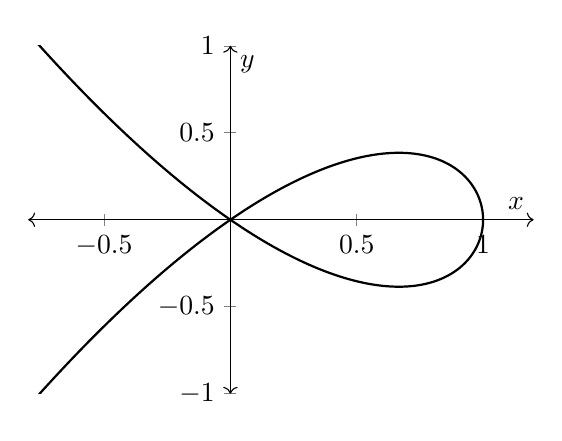
\begin{tikzpicture}
				\begin{axis}[
					height=6cm,
					width=8cm,
					xmin=-.8,xmax=1.2,
					ymin= -1,ymax=1,
					]
					\addplot [domain=-2:2,samples=1000, thick]({1-x^2},{x*(1-x^2)}); 
				\end{axis}
			\end{tikzpicture}
		\end{center}
		Then $M$ is not a $1$-dimensional manifold.\\
		\textbf{Hint:} connected components
	\end{ex}

	\begin{proof}
		Suppose that $M$ is a $1$-dimensional manifold. Set $p = (0,0)$. Then there exists $(U, \phi) \in X(M)$ such that $p \in U$. Since $\phi(U)$ is open (in $\R$ or $\H$), there exists a $B \subset \phi(U)$ such that $B$ is open (in $\R$ or $\H$), $B$ is connected and $\phi(p) \in B$. Set $V = \phi^{-1}(B)$, $V' = V \setminus \{p\}$ and $B' = B \setminus \{\phi(p)\}$. Then $\phi: V \rightarrow B$ and $\phi': V' \rightarrow B'$ are homeomorphisms. Since $B$ is open (in $\R$ or $\H$) and connected, $B'$ has at most two connected components. Then $V'$ This is a contradiction since $V'$ has four connected components and $B'$ and $V'$ are homeomorphic. 
	\end{proof}













	
	
	
	
	
	
	
	
	
	
	
	
	\newpage
	\subsection{Smooth Manifolds}

	\begin{defn}
		Let $M$ be an $n$-dimensional manifold and $(U, \phi), (V, \psi) \in X(M)$. Then $(U, \phi)$ and $(V, \psi)$ are said to be \textbf{smoothly compatible} if $$\phi \circ \psi^{-1}: \psi(U \cap V) \rightarrow \phi (U \cap V) \text{ is a diffeomorphism}$$ 
	\end{defn}

	\begin{defn} Let $M$ be an $n$-dimensional manifold.
		\begin{enumerate}
			\item Let $\MA \subset X(M)$. Then $\MA$ is said to be an \textbf{atlas on $M$} if  $\bigcup\limits_{(U,\phi) \in \MA} U = M$.
			\item Let $\MA$ be an atlas on $M$. Then $\MA$ is said to be \textbf{smooth} if for each $(U, \phi), (V, \psi) \in \MA$, $(U,\phi)$ and $(V,\psi)$ are smoothly compatible.
			\item Let $\MA$ be a smooth atlas on $M$. Then $\MA$ is said to be \textbf{maximal} if for each smooth atlas $\MB$ on $M$, $\MA \subset \MB$ implies that $\MA = \MB$. A maximal smooth atlas on $M$ is called a \textbf{smooth structure on $M$}.
			\item Let $\MA$ be an atlas on $M$. Then $(M, \MA)$ is said to be an \textbf{$n$-dimensional smooth manifold} if $\MA$ is a smooth structure on $M$. 
		\end{enumerate}
	\end{defn}

	\begin{ex}
		Let $M$ be a topological space and $\MB$ a smooth atlas on $M$. Then there exists a unique smooth structure $\MA$ on $M$ such that $\MB \subset \MA$.
	\end{ex}

	\begin{proof}
		Define $\MA$ to be the set of all coordinate charts $(U, \phi)$ on $M$ such that for each coordinate chart $(V, \psi) \in \MB$,  $(U, \phi)$ and $(V, \psi) $ are smoothly compatible. \\
		Clearly $\MB \subset \MA$. \\
		Let $(U, \phi), (V, \psi) \in \MA$ and $p \in U \cap V$. Then there exists $(W, \chi) \in \MB$ such that $p \in W$. By assumption, $\phi \circ \chi^{-1} : \chi(U \cap W) \rightarrow \phi(U \cap W)$ and $ \chi \circ \psi^{-1} : \psi(W \cap V) \rightarrow \chi(W \cap V)$ are diffeomorphisms. Then $ (\phi \circ \chi^{-1}) \circ (\chi \circ \psi^{-1}) = \phi \circ \psi^{-1}: \psi(U \cap W \cap V) \rightarrow  \phi(U \cap W \cap V) $ is a diffeomorphism.  Since for each $q \in \psi(U \cap V)$, there exits an open neighborhood $N \subset \psi(U \cap V)$ of $q$ on which $\phi \circ \psi^{-1}$ are diffeomorphic, we have that $\phi \circ \psi^{-1}$ is a diffeomorphism on $\psi(U \cap V)$ and therefore $(U, \phi)$ and $ (V, \psi)$ are smoothly compatible. Hence $\MA$ is a smooth atlas.\\
		To see that $\MA$ is maximal, let $\MB'$ be a smooth atlas on $M$. Suppose that $\MA \subset \MB'$ and let $(U, \phi) \in \MB'$. By definition, for each chart $(V, \psi) \in \MB'$, $(U, \phi)$ and $(V, \psi)$ are smoothly compatible. Since $\MB \subset \MA \subset \MB'$, we have that $(U, \phi) \in \MA$. So $\MA = \MB'$ and $\MA$ is a maximal smooth atlas on $M$.
	\end{proof}

	\begin{ex}
		Let $(M, \MA)$ be a $n$-dimensional smooth manifold, $(U, \phi) \in \MA$ and $U' \subset U$. Define $\phi': U' \rightarrow \phi(U')$ by $\phi' = \phi|_{U'}$. Then $(U', \phi') \in \MA$. 
	\end{ex}

	\begin{proof}
		Clearly $(U', \phi') \in X(M)$. Let $(V, \psi) \in \MA$. Then $\phi \circ \psi: \psi(U \cap V) \rightarrow \phi(U \cap V)$ is a diffeomorphism. Since $U' \subset U$, $\phi \circ \psi: \psi(U' \cap V) \rightarrow \phi(U' \cap V)$ is a diffeomorphism. Since $\phi \circ \psi = \phi' \circ \psi$ on $U' \cap V$, $\phi' \circ \psi$ is a diffeomorphism. Therefore $(U', \phi')$ and $(V, \psi)$ are smoothly compatible. Since $(V, \psi) \in \MA$ is arbitrary, and $\MA$ is maximal, $(U', \phi') \in \MA$.
	\end{proof}

	\begin{defn}
		Let $(M, \MA)$ be a smooth $n$-dimensional manifold and $U \subset M$ open. We define $\MA|_{U} = \{(U', \phi') \in \MA: U' \subset U\}$. 
	\end{defn}

	\begin{ex} \textbf{Smooth Open Submanifold:} \\
		Let $(M, \MA)$ be a smooth $n$-dimensional manifold and $U \subset M$ open. Then 
		\begin{enumerate}
			\item $\MA|_{U}$ is a smooth structure on $U$
			\item $(U, \MA|_{U})$ is an smooth $n$-dimensional manifold
			\item $\p U = \p M \cap U$
		\end{enumerate}
	\end{ex}

	\begin{defn} 
		Let $(M, \MA)$ be a $n$-dimensional smooth manifold. Define $\pi: \p \H^n \rightarrow \R^{n-1}$ by 
		$$\pi(x_1, \ldots, x_{n-1}, 0) = (x_1, \ldots, x_{n-1})$$
		For $(U, \phi) \in \MA$, set $\bar{U} = U \cap \p M$ and $\bar{\phi} = \pi \circ \phi|_{\bar{U}}$. \\
		Define $\MA|_{\p M} = \{(\bar{U}, \bar{\phi}): (U, \phi) \in \MA \text{ and } U \cap \p M \neq \varnothing \}$.
	\end{defn}
	
	\begin{ex}
		Let $(M, \MA)$ be a $n$-dimensional smooth manifold. Then 
		\begin{enumerate}
			\item $\MA|_{\p M}$ is a smooth structure on $\p M$  
			\item $(\p M, \MA|_{\p M})$ is a $(n-1)$-dimensional smooth manifold
			\item $\partial (\partial M) = \varnothing$
		\end{enumerate}
	\end{ex}
	
	\begin{proof} \
		\begin{enumerate}
			\item A previous exercise implies that $\pi$ is a homeomorphism and it is clear that $\pi$ is a diffeomorphism. Let $p \in \partial M$. Then there exists a boundary chart $(U, \phi)$ on $M$ such that $p \in U$. Thus $p \in \bar{U}$ and the previous exercise implies that 
				\begin{align*}
				\phi(\bar{U}) 
				& = \phi (U \cap \p M) \\
				& = \phi(U) \cap \p \H^n 
			\end{align*}
			Since $U$ is open in $M$ and $\phi(U)$ is open in $\H^n$, we have that $\bar{U}$ is open in $\p M$ and $\phi(\bar{U})$ is open in $\p \H^n$ which implies that $\pi(\phi(\bar{U}))$ is open in $\R^{n-1}$. Since $\phi: U \rightarrow \phi(U)$ is a homeomorphism, $\phi|_{\bar{U}}: \bar{U} \rightarrow \phi(\bar{U})$ is a homeomorphism. Hence $\bar{\phi}: \bar{U} \rightarrow \pi(\phi(\bar{U}))$ is a homeomorphism and $(\bar{U}, \bar{\phi})$ is an interior chart on $\p M$. Therefore $\MA|_{\p M }$ is an atlas on $\p M$. Let $(\bar{U}, \bar{\phi})$, $(\bar{V}, \bar{\psi}) \in \MA|_{\p M}$. Then 
			\begin{align*}
				\bar{\phi} \circ \bar{\psi}^{-1}
				& = \pi \circ \phi \circ \psi^{-1} \circ \pi^{-1}
			\end{align*}
			which is a diffeomorphism. So $(\bar{U}, \bar{\phi})$ and $(\bar{V}, \bar{\psi})$ are smoothly compatible. Hence $\MA$ is smooth.
			\\
			\item Subspaces of Hausdorff, second countable spaces are Hausdorff and second countable, so $\p M$ with the subspace topology is Hausdorff and second countable. Since  $\MA|_{\p M }$ is an atlas on $\p M$, $(\p M,  \MA|_{\p M })$ is and $(n-1)$-dimensional manifold. \\
			\item Since for each $(\bar{U}, \bar{\phi}) \in \MA|_{\p M}$, $\bar{\phi}(\bar{U})$ is open in $\R^n$, $(\bar{U}, \bar{\phi})$ is an interior chart. Hence $\p(\p M) = \varnothing$.
		\end{enumerate}
	\end{proof}

	
	
	\begin{note}
		For the rest of this section, we assume that $(M, \MA)$ is a $n$-dimensional smooth manifold and we denote the standard coordinate functions on $\R^n$ by $u^1, \cdots, u^n$. For a coordinate chart $(U, \phi)$ $\in \MA$ and $i \in \{1, \cdots, n\}$, we will typically denote the $i$th coordinate of $\phi$ by $x^i$, that is,  $x^i = u^i(\phi)$.
	\end{note}
	
	
	
	
	
	
	
	
	
	
	
	
	
	
	\begin{ex}
	Let $(M, \MA)$ be a $n$-dimensional smooth manifold and $S \subset M$ open. For $(U, \phi) \in \MA$, define $U' \subset S$ and $\phi': \tilde{U} \rightarrow \phi(U')$ by $U' = U \cap S$ and $\phi' = \phi|_{U \cap S}$. Set $\MA' = \{(U', \phi'): (U, \phi) \in \MA\}$.
	Then $(S, \MA')$ is a $n$-dimensional smooth manifold. 
	\end{ex}
	
	\begin{proof}
	Since $M$ is Hausdorff and second countable, so is $S$. Clearly $S= \bigcup\limits_{(U', \phi') \in \MA'} U'$ and for each $(U', \phi') \in \MA'$, $\phi'$ is a homeomorphism and $\phi'(U') \subset \H^n$. Let $(U', \phi'), (V', \psi') \in \MA'$. Then there exist $(U, \phi)$, $(V, \psi) \in \MA$ such that $U' = U \cap S$, $V' = V \cap S$. Then $\psi' \circ \phi'^{-1}: \phi(U \cap V \cap S) \rightarrow \psi(U \cap V \cap S)$ is given by 
	\begin{align*}
	\psi' \circ \phi'^{-1}: \phi(U' \cap V') \rightarrow \psi(U' \cap V')
	&= \psi \circ \phi^{-1}: \phi(U \cap V \cap S) \rightarrow \psi(U \cap V \cap S)
\end{align*}	 
which is smooth. So $\MA'$ is a smooth atlas. Let $\MB'$ be a smooth atlas on $S$. Suppose that $\MA' \subset \MB'$.
	\end{proof}

\begin{ex}
	Let $(M, \MA)$ a smooth manifold an $U \subset M$ open. For $(V, \psi) \in \MA$, define $\bar{V} \subset M $ and $ \bar{\psi}: \bar{V} \rightarrow \psi(\bar{V})$ by $\bar{V} = V \cap U$ and $\bar{\psi} = \psi|_{V \cap U}$. Define $$\MA \cap U = \{(\bar{V}, \bar{\psi}): (V, \psi) \in \MA\}$$ Then 
	\begin{enumerate}
		\item $\MA_U$ is an atlas on $U$
		\item $\MA_U$ is a smooth structure on $U$ 
		\item $(U, \MA_U)$ is an $n$-dimensional smooth manifold.
	\end{enumerate}
\end{ex}

\begin{defn}
	Let $(M, \MA)$ an $n$-dimensional smooth manifold an $U \subset M$ open. Define $(U, \MA_U)$ as in the previous exercise. 
\end{defn}	
	
	
	
	
	
	
	
	
	
	
	
	
	
	
	
	
	\newpage 
	\subsection{Smooth Maps}	
	
	\begin{defn} \ld{42001}
		Let $f: M \rightarrow \R$. Then $f$ is said to be smooth if for each coordinate chart $(U, \phi) \in \MA$, $f \circ \phi^{-1}$ is smooth. The set of all smooth functions on $M$ is denoted $C^{\infty}(M)$. 
	\end{defn}

	\begin{ex} \ld{42002}
		We have that $C^{\infty}(M)$ is a vector space.
	\end{ex}

	\begin{proof}
		Clear.
	\end{proof}
	
	\begin{defn} \ld{42003}
	Let $(M, \MA)$ be a smooth manifold, $(U, \phi) \in \MA$. We define $$C^{\infty}(U) = \{f:U \rightarrow \R: f \circ \phi^{-1} \in C^{\infty}(\phi(U))\}$$
	\end{defn}
	
	\begin{note}
	Later we will give a subset $S \subset M$ the structure of a smooth manifold such that \rd{42001} and \rd{42003} coincide.
	\end{note}
	
	\begin{ex}
	Let $(M, \MA)$ be a smooth manifold, $(U, \phi) \in \MA$ with $\phi = (x^1, \cdots, x^n)$, $p \in U$ and $f \in C^{\infty}(M)$. Then $f|_U \in C^{\infty}(U)$.
	\end{ex}
	
	\begin{proof}\
	\textbf{FINISH!!!}
	\end{proof}
	
	\begin{defn}
	Let $(M, \MA)$ be a smooth manifold, $(U, \phi) \in \MA$ with $\phi = (x^1, \cdots, x^n)$, $f \in C^{\infty}(U)$ and $i \in \{1, \cdots, n\}$. We define the \textbf{partial derivative of $f$ with respect to $x^i$}, denoted $$ \p f / \p x^i: U \rightarrow \R \hspace{.1cm} \text{ or } \hspace{.1cm} \p_{i} f: U \rightarrow \R$$ by 
	\begin{equation*}
	{\pdv{f}{x^i}}(p) = {\pdv{u^i}[f \circ \phi^{-1}] }( \phi(p)) 
	\end{equation*}
	or equivalently,
	\begin{equation*}
	{\pdv{f}{x^i}} = \bigg({\pdv{u^i}[f \circ \phi^{-1}] \bigg) \circ \phi }
	\end{equation*}
	\end{defn}
	
	\begin{ex}
	Let $(M, \MA)$ be a smooth manifold, $(U, \phi) \in \MA$ with $\phi = (x^1, \cdots, x^n)$, $f \in C^{\infty}(U)$ and $i \in \{1, \cdots, n\}$. Then $\p / \p x^i:  C^{\infty}(U) \rightarrow C^{\infty}(U)$ is linear.
	\end{ex}
	
	\begin{proof}
	\textbf{FINISH!!!}
	\end{proof}
	
	\begin{ex}
	Let $(M, \MA)$ be a smooth manifold, $(U, \phi) \in \MA$ with $\phi = (x^1, \cdots, x^n)$, $f \in C^{\infty}(U)$ and $i,j \in \{1, \cdots, n\}$. Then 
	$$ \pdv{x^i} \pdv{x^j} f =  \bigg(\pdv{u^i} \pdv{u^j}[f \circ \phi^{-1}] \bigg) \circ \phi $$
	\end{ex}
	
	\begin{proof}
	
	\begin{align*}
	\pdv{x^i} \pdv{x^j} f 
	&= \pdv{x^i} \bigg( \pdv{x^j} f \bigg) \\
	&= \pdv{x^i} \bigg( \bigg[\pdv{u^j} [f \circ \phi^{-1}] \bigg] \circ \phi \bigg) \\
	&=  \bigg( \pdv{u^i} \bigg[ \bigg( \bigg[\pdv{u^j} [f \circ \phi^{-1}] \bigg] \circ \phi \bigg) \circ \phi^{-1} \bigg] \bigg) \circ \phi \\
	&= \bigg( \pdv{u^i} \bigg[\pdv{u^j} [f \circ \phi^{-1}] \bigg]  \bigg) \circ \phi \\
	&= \bigg( \pdv{u^i} \pdv{u^j} [f \circ \phi^{-1}]  \bigg) \circ \phi \\
	\end{align*}
	\end{proof}
	
	\begin{ex}
	Let $(M, \MA)$ be a smooth manifold, $(U, \phi) \in \MA$ with $\phi = (x^1, \cdots, x^n)$ and $i,j \in \{1, \cdots, n\}$. Then 
	\begin{equation*}
	\pdv{x^i}\pdv{x^j} = \pdv{x^j}\pdv{x^i}
	\end{equation*}
	\end{ex}
	
	\begin{proof}
	Let $f \in C^{\infty}(U)$. Since $f \circ \phi^{-1}$ is smooth, $$\pdv{u^i} \pdv{u^j} [f \circ \phi^{-1}] = \pdv{u^j} \pdv{u^i} [f \circ \phi^{-1}] $$
	The previous exercise implies that 
	
	\begin{align*}
	\pdv{x^i}\pdv{x^j}f 
	&= \bigg( \pdv{u^i} \pdv{u^j} [f \circ \phi^{-1}]  \bigg) \circ \phi \\
	&= \bigg( \pdv{u^j} \pdv{u^i} [f \circ \phi^{-1}]  \bigg) \circ \phi \\
	&= \pdv{x^j}\pdv{x^i}f 
	\end{align*}
	\end{proof}
	
	\begin{ex}
	Let $(M, \MA)$ be a smooth manifold, $(U, \phi) \in \MA$ with $\phi = (x^1, \cdots, x^n)$ and $f \in C^{\infty}(U)$. Then for each $\al \in \N_0^n$, $$\p^{\al} f = (\p^{\al}[ f \circ \phi^{-1}] ) \circ \phi$$
	\end{ex}	
	
	\begin{proof}
	The claim is clearly true when $|\al| =0$ or by definition if $|\al| = 1$. Let $n \in \N$ and suppose the claim is true for each $|\al| \in \{1, \ldots, n-1 \}$. Then there exists $i \in \{1, \ldots, n\}$ such that $\al_i \geq 1$. Hence 
	\begin{align*}
	\p^{\al}f 
	&= \p^{e^i} (\p^{\al - e^i} f) \\
	&= \p^{e^i} (\p^{\al - e^i}[ f \circ \phi^{-1}] \circ \phi) \\
	&= (\p^{e^i} [(\p^{\al - e^i}[ f \circ \phi^{-1}] \circ \phi) \circ \phi^{-1} ]) \circ \phi\\
	&= (\p^{e^i} [\p^{\al - e^i}[ f \circ \phi^{-1}]] )\circ \phi\\
	&= (\p^{\al}[ f \circ \phi^{-1}] )\circ \phi\\
	\end{align*}
	\end{proof}
	
	
	\begin{ex} \textbf{Taylor's Theorem:} \\
	Let $(M, \MA)$ be a smooth manifold, $(U, \phi) \in \MA$ with $\phi = (x^1, \ldots, x^n)$ and $\phi(U)$ convex, $p \in U$, $f \in C^{\infty}(U)$ and $T \in \N$. Then there exist $(g_{\al})_{|\al| = T+1} \subset C^{\infty}(U)$ such that
		$$f = \sum_{k=0}^{T} \bigg[\sum_{|\al| = k}(x - p)^{\al} \p^{\al} f (x_0) \bigg] + \sum_{|\al| = T+1}(x^i - x^i(p))^{\al} g_{\al}$$ and for each $|\al|= T+1$, $$g_{\al}(p) = \frac{1}{(T+1)!}\p^{\al} f(p)$$
	\end{ex}
	
	\begin{proof}
	Since $\phi(U)$ is open and convex and $f \circ \phi^{-1} \in C^{\infty}(\phi(U))$, Taylors thorem in section $2.1$ implies that there exist $(\tilde{g}_{\al})_{|\al| = T+1} \subset C^{\infty}(\phi(U))$ such that for each $q \in U$, 
	$$f \circ \phi^{-1} (\phi(q)) = \sum_{k=0}^{T} \bigg[\sum_{|\al| = k}(x^i(q) - x^i(p))^{\al} \p^{\al} [f \circ \phi^{-1}] (\phi(p)) \bigg] + \sum_{|\al| = T+1}(x^i(q) - x^i(p))^{\al} \tilde{g}_{\al}(\phi(q)) $$	
		and for each $|\al|= T+1$, 
		\begin{align*}
		\tilde{g}_{\al}(\phi(p)) 
		&= \frac{1}{(T+1)!}\p^{\al} [f \circ \phi^{-1}](\phi(p)) \\
		&= \frac{1}{(T+1)!}\p^{\al} f (p)
		\end{align*}
		For $|\al| = T+1$, set $g_{\al} = \tilde{g} \circ \phi$. Then 
		\begin{align*}
	f(q) 
	&= f \circ \phi^{-1} (\phi(q)) \\
	&= \sum_{k=0}^{T} \bigg[\sum_{|\al| = k}(x^i(q) - x^i(p))^{\al} \p^{\al} [f \circ \phi^{-1}] (\phi(p)) \bigg] + \sum_{|\al| = T+1}(x^i(q) - x^i(p))^{\al} \tilde{g}_{\al}(\phi(q)) \\
	&= \sum_{k=0}^{T} \bigg[\sum_{|\al| = k}(x^i(q) - x^i(p))^{\al} \p^{\al} f(p) \bigg] + \sum_{|\al| = T+1}(x^i(q) - x^i(p))^{\al} g_{\al}(q) \\
\end{align*}			
	\end{proof}

	\begin{defn}
		Let $(N, \MB)$ be a smooth manifold and $F: M \rightarrow N$. Then $F$ is said to be 
		\begin{itemize}
		\item \textbf{smooth} if for each $(U, \phi) \in \MA$ and $(V, \psi) \in \MB$, $$\psi \circ F \circ \phi^{-1}: \phi(U \cap F^{-1}(V)) \rightarrow \psi(F(U) \cap V)$$ is smooth 
		\item a \textbf{diffeomorphism} if $F$ is a bijection and $F,F^{-1}$ are smooth.
		\end{itemize}
	\end{defn}
	
	\begin{ex}
	Let $(M, \MA)$ and $(N, \MB)$ be smooth manifold and $F: M \rightarrow N$. If $F$ is smooth, then $F$ is continuous. 
	\end{ex}
	
	\begin{proof}
	Suppose that $F$ is smooth. Let $p \in M$. Choose $(U, \phi) \in \MA$ and $(V, \psi) \in \MB$ such that $p \in U$ and $F(p) \in V$. Put $\tU = U \cap F^{-1}(V)$ and $\tV = F(U) \cap V$. \\
	Define $\tphi: \tU \rightarrow \phi(\tU)$ and $\tpsi: \tV \rightarrow \psi(\tV)$ by $$\tphi = \phi|_{\tU}, \hspace{.2cm} \tphi = \psi|_{\tV}$$ Then $\tphi$ and $\tpsi$ are homeomorphisms, $p \in \tU$ and $F(\tU) \subset \tV$. Define $\tF: \phi(\tU) \rightarrow \psi(\tV) $ by $$ \tF = \tpsi \circ F \circ \tphi^{-1}$$  
	By definition, $\tF$ is smooth and therefore continuous. Since $\phi$ and $\psi$ are homeomorphisms and $F|_{\tU} = \tpsi^{-1} \circ \tF \circ \tphi$, we have that $F|_{\tU}$ is continuous. In particular, $F$ is continuous at $p$ and since $p \in M$ is arbitrary, $F$ is continuous.
	\end{proof}
	
	\begin{ex}
	Let $(M, \MA)$ and $(N, \MB)$ be smooth manifold and $F: M \rightarrow N$. If $F$ is a diffeomorphism, then $F$ is a homeomorphism. 
	\end{ex}	
	
	\begin{proof}
	Suppose that $F$ is a diffeomorphism. By definition, $F$ and  $F^{-1}$ are smooth. The previous exercise implies that $F$ and $F^{-1}$ are continuous. Hence $F$  is a homeomorphism. 
	\end{proof}
	
	\begin{ex}
		Let $(N, \MB)$ be a smooth manifold and $F: M \rightarrow N$ a diffeomorphism. Then for each $(U, \phi) \in \MA$, $(F(U), \phi \circ F^{-1}) \in \MB$.
	\end{ex}
	
	\begin{proof}
		Let $(V, \psi) \in \MB$. 
		\begin{enumerate}
		\item Since $\phi$ and $F^{-1}$ are homeomorphisms, $\phi \circ F^{-1}: F(U) \cap V \rightarrow \phi(U \cap F^{-1}(V))$ is a homeomorphism
		\item Since $F$ is a diffeomorphism, $$\phi \circ F^{-1} \circ \psi^{-1}: \psi(F(U) \cap V) \rightarrow \phi(U \cap F^{-1}(V))$$ and $$\psi \circ F \circ \phi^{-1}: \phi(F^{-1}(V) \cap U) \rightarrow \psi(V \cap F(U))$$ are smooth. 
		\end{enumerate}
		
		Therefore $(F(U), \phi \circ F^{-1})$ and $(V, \psi)$ are smoothly compatible. Since $\MB$ is maximal, $(F(U), \phi \circ F^{-1}) \in \MB$.
	\end{proof}


	\begin{defn}
		Let $(N, \MB)$ be a smooth  $n$-dimensional manifold, $F: M \rightarrow N$ smooth and $(V, \psi) \in \MB$ with $\psi = (y^1, \dots, y^n)$. For $i \in \{1, \dots, n\}$, We define the \textbf{$i$-th component of $F$ with respect to $(V, \psi)$},  denoted $F^i: V \rightarrow \R$, by $$F^i = y^i \circ F$$  
	\end{defn}

	











\newpage 
\subsection{Partitions of Unity}
	
	\begin{defn}
	Let $p \in M$, $U \in \MN_a$ open and $\rho \in C_c^{\infty}(M)$. Then $\rho$ is said to be a \textbf{bump function at p supported in $U$} if 
	\begin{enumerate}
	\item $\rho \geq 0$ 
	\item there exists $V \in \MN_p$ such that $V$ is open and $\rho|_V = 1$ 
	\item $\supp \rho \subset U$
	\end{enumerate}
	\end{defn}
	
	\begin{ex}
	Define $f:\R \rightarrow \R$ by 
	\[
	f(t) = 
	\begin{cases}
	e^{-\frac{1}{1-t^2}} & t \in (-1,1)\\
	0 &  t \not \in (-1,1)
	\end{cases}
	\]
	Then $f \in C_c^{\infty}(\R)$.
	\end{ex}
	
	\begin{proof}
	
	\end{proof}
	
	
















	\newpage
	\subsection{The Tangent Space}

	\begin{defn}
		Let $p \in M$. Define the relation $\sim_p$ on $C^{\infty}(M)$ by $f \sim_p g$ iff there exists $U \in \MN_p$ such that $U$ is open and $f|_U = g|_U$. Clearly $\sim_p$ is an equivalence relation on $C^{\infty}(M)$. We denote $C^{\infty}(M) / \sim_p$ by $C^{\infty}_p(M)$. For $f \in C^{\infty}(M)$, we define the \textbf{germ of $f$ at $p$} to be the equivalence class of $f$ under $\sim_p$. 
	\end{defn}
	
	\begin{ex}
		Let $p \in $We have that $C_p^{\infty}(M)$ is a vector space.
	\end{ex}
	
	\begin{proof}
		Clear.
	\end{proof}

	\begin{defn}
		Let $(U, \phi) \in \MA$ with $\phi = (x^1, \cdots, x^n)$ and $p \in U$. For $i \in \{1, \cdots, n\}$, define the partial derivative with respect to $x^i$ at $p$, denoted $$\eval{\pdv{x^i}}_{p}: C_p^{\infty}(M) \rightarrow \R  \text{, or } \p_i|_p: C_p^{\infty}(M) \rightarrow \R $$ by $$ \eval{\pdv{x^i}}_{p} f =  {\pdv{f}{x^i}}(p) $$
	\end{defn}

	\begin{ex}
		Let $(U, \phi) \in \MA$ with $\phi = (x^1, \cdots, x^n)$ and $p \in U$. Then for each $i,j \in \{1, \cdots, n\}$, we have that $${\pdv{x^i}{x^j}}(p) = \del_{i,j}$$
	\end{ex}

	\begin{proof}
		Let $i,j \in \{1, \cdots, n\}$. Then 
		\begin{align*}
			\eval{\pdv{x^j}}_{p} x^i 
			&=  \eval{\pdv{u^j}}_{\phi(p)} x^i \circ \phi^{-1} \\
			&= \eval{\pdv{u^j}}_{\phi(p)} u^i \circ \phi \circ \phi^{-1} \\
			&= \eval{\pdv{u^j}}_{\phi(p)} u^i  \\
			&= \del_{i,j}
		\end{align*}
	\end{proof}

	\begin{ex} \textbf{Change of Coordinates:}\\
		Let $(U, \phi), (V, \psi) \in \MA$ with $\phi = (x^1, \cdots, x^n)$ and $\psi = (y^1, \cdots, y^n)$, $p \in U \cap V$ and $f \in C_p^{\infty}(M)$. Then for each $i \in \{1, \cdots, n\}$, 
		 $$\eval{\pdv{y^i}}_{p} = \sum_{j =1}^n {\pdv{x^j}{y^i}}(p) \eval{\pdv{x^j}}_{p}    $$
	\end{ex}

	\begin{proof}
		Put $h = \phi \circ \psi^{-1}$ and write $h = (h_1, \cdots, h_n)$. Then $\phi = h \circ \psi$ and $\psi^{-1} = \phi^{-1} \circ h$. By definition and the chain rule, we have that 
		\begin{align*}
		\eval{\pdv{y^i}}_{p} f 
			&= \eval{\pdv{u^i}}_{\psi(p)} f \circ \psi^{-1} \\
			&= \eval{\pdv{u^i}}_{\psi(p)} f \circ \phi^{-1} \circ h \\
			&= \sum_{j=1}^n \bigg( \eval{\pdv{u^j}}_{h \circ \psi (p)} f \circ \phi^{-1} \bigg)  \bigg( \eval{\pdv{u^i}}_{\psi(p)} h_j \bigg) \\
			&= \sum_{j=1}^n \bigg( \eval{\pdv{u^j}}_{\phi (p)} f \circ \phi^{-1}  \bigg) \bigg( \eval{\pdv{u^i}}_{\psi(p)} x^j \circ \psi^{-1} \bigg) \\
			&= \sum_{j=1}^n \bigg( \eval{\pdv{x^j}}_{p} f \bigg)  \bigg(   \eval{\pdv{y^i}}_{p} x^j  \bigg)\\
		\end{align*}
	\end{proof}

	\begin{defn}
		Let $p \in M$ and $v: C^{\infty}_p(M) \rightarrow \R$. Then $v$ is said to be \textbf{Leibnizian} if for each $f,g \in  C^{\infty}_p(M)$, $$v(fg) = v(f)g(p) + f(p)v(g)$$ and $v$ is said to be a \textbf{derivation at $p$} if for each $f, g \in C^{\infty}_p(M)$ and $a \in \R$,
		\begin{enumerate}
			\item $v$ is linear 
			\item $v$ is Leibnizian
		\end{enumerate}
		We define the \textbf{tangent space of $M$ at $p$}, denoted $T_pM$, by $$T_pM = \{ v: C^{\infty}_p(M) \rightarrow \R: v \text{ is a derivation at }p\}$$
	\end{defn}

	\begin{ex}
		Let $f \in C^{\infty}_p(M)$ and $v \in T_pM$. If $f$ is constant, then $vf = 0$.
	\end{ex}

	\begin{proof}
		Suppose that $f = 1$. Then $f^2 = f$ and $v(f^2) = 2v(f)$. So $v(f) = 2v(f)$ which implies that $v(f) = 0$. If $f \neq 1$, then there exists $c \in \R$ such that $f = c$. Since $v$ is linear, $v(f) = cv(1) = 0$.
	\end{proof}

	\begin{ex}
		Let $(U, \phi) \in \MA$ with $\phi = (x^1, \cdots, x^n)$ and $p \in U$. Then $$ \bigg \{\eval{\pdv{x^1}}_{p}, \cdots, \eval{\pdv{x^n}}_{p} \bigg \}$$ is a basis for $T_pM$ and $\dim T_pM = n$.
	\end{ex}

	\begin{proof}
		Clearly $\eval{\pdv{x^1}}_{p}, \cdots, \eval{\pdv{x^n}}_{p} \in T_pM$. Let $a_1, \cdots, a_n \in \R$. Suppose that $$v = \sum_{i=1}^n a_i \eval{\pdv{x^i}}_{p} = 0$$
		Then 
		\begin{align*}
			0
			&= v x^j \\
			&= \sum_{i=1}^n a_i \eval{\pdv{x^i}}_{p} x^j \\
			&= a_j
		\end{align*}
		Hence $\bigg \{\eval{\pdv{x^1}}_{p}, \cdots, \eval{\pdv{x^n}}_{p} \bigg \}$ is independent.\\
		Now, let $v \in T_pM$ and $f \in \C^{\infty}_p(M)$. By Taylor's theorem, there exist $g_1, \cdots g_n \in C_p^{\infty}(M)$ such that $$f = f(p) + \sum_{i=1}^n(x^i - x^i(p)) g_i$$ and for each $i \in \{1, \cdots, n\}$, $$g_i(p) = \eval{\pdv{x^i}}_{p} f $$ Then 
		\begin{align*}
			v(f)
			&= \sum_{i=1}^nv(x^i - x^i(p)) g_i(p) + \sum_{i=1}^n(x^i(p) - x^i(p)) v(g_i) \\
			&= \sum_{i=1}^nv(x^i)g_i(p) \\
			&= \sum_{i=1}^nv(x^i)\eval{\pdv{x^i}}_{p} f \\
			&= \bigg[ \sum_{i=1}^nv(x^i)\eval{\pdv{x^i}}_{p} \bigg] f
		\end{align*}
		So $$v = \sum_{i=1}^nv(x^i)\eval{\pdv{x^i}}_{p} $$ and $$v \in \spn \bigg \{\eval{\pdv{x^1}}_{p}, \cdots, \eval{\pdv{x^n}}_{p} \bigg \}$$
	\end{proof}



	\begin{defn}
		Let $(N, \MB)$ be a smooth manifold, $F: M \rightarrow N$ smooth and $p \in M$. We define the \textbf{differential of $F$ at $p$}, denoted $dF_p: T_pM \rightarrow T_{F(p)}N$, by $$\bigg[ dF_p(v) \bigg] (f) = v (f \circ F)$$  for $v \in T_pM$ and $f \in C^{\infty}_{F(p)}(N)$.
	\end{defn}
	
	
	
	\begin{ex}
	Let $(N, \MB)$ be a smooth manifold, $F: M \rightarrow N$ smooth and $p \in M$. Then for each $v \in T_pM$, $dF_p(v)$ is a derivation.
	\end{ex}
	
	\begin{proof}
	Let $v \in T_pM$, $f,g \in C_{F(p)}^{\infty}(N)$ and $c \in \R$. Then 
	\begin{enumerate}
	\item 
	\begin{align*}
		dF_p(v)(f+cg) 
		&= v((f+cg) \circ F) \\
		&= v(f \circ F + c g \circ F) \\
		&= v(f \circ F) + cv(g \circ F) \\
		&= dF_p(v)(f) + c dF_p(v)(g)
	\end{align*}
	So $dF_p(v)$ is linear.
	\item 
	\begin{align*}
	dF_p(v)(fg) 
	&= v (fg \circ F) \\
	&= v((f \circ F)* (g \circ F)) \\
	&= v(f \circ F)*(g \circ F)(p) +  (f \circ F)(p)* v(g \circ F) \\
	&= dF_p(v)(f) * g(F(p)) + f(F(p))*dF_p(v)(g) \\
	\end{align*}
	\end{enumerate}
	So $dF_p(v)$ is Leibnizian and hence $dF_p(v) \in T_{F(p)}N$
	\end{proof}

	\begin{ex}
		Let $(N, \MB)$ be a smooth manifold, $F: M \rightarrow N$ smooth and $p \in M$. If $F$ is a diffeomorphism, then $dF_p$ is an isomorphism.
	\end{ex}
	
	\begin{proof}
		Suppose that $F$ is a diffeomorphism. Since $F$ is a homeomorphism, $\dim N = n$. Choose $(U, \phi) \in \MA$ such that $p \in U$. A previous exercise tells us that $(F(U), \phi \circ F^{-1}) \in \MB$. Write $\phi = (x^1, \cdots, x^n)$ and $\phi \circ F^{-1} = (y^1, \cdots, y^n)$. Let $f \in C^{\infty}_{F(p)}(N)$ Then 
		\begin{align*}
			\eval{\pdv{y^i}}_{F(p)} f
			&= 	\eval{\pdv{u^i}}_{\phi \circ F^{-1} (F(p))} f \circ (\phi \circ F^{-1})^{-1} \\
			&= 	\eval{\pdv{u^i}}_{\phi(p)} f \circ F \circ \phi^{-1} \\
			&= 	\eval{\pdv{x^i}}_p f \circ F \\
		\end{align*}
		Therefore 
		\begin{align*}
			\bigg[ dF_p \bigg( \eval{\pdv{x^i}}_p \bigg) \bigg] (f)
			&= \eval{\pdv{x^i}}_p f \circ F \\
			&= \eval{\pdv{y^i}}_{F(p)} f 
		\end{align*}
	Hence $$dF_p \bigg( \eval{\pdv{x^i}}_p \bigg) = \eval{\pdv{y^i}}_{F(p)}$$ 
	Since $\bigg \{\eval{\pdv{x^1}}_{p}, \cdots, \eval{\pdv{x^n}}_{p} \bigg \}$ is a basis for $T_pM$ and $\bigg \{\eval{\pdv{y^1}}_{F(p)}, \cdots, \eval{\pdv{y^n}}_{F(p)} \bigg \}$ is a basis for $T_{F(p)}N$, $dF_p$ is an isomorphism.
	\end{proof}

	\begin{ex}
		Let $(M, \MA)$ be a smooth $m$-dimensional manifold, $(N, \MB)$ a $n$-dimensional smooth manifold, $F: M \rightarrow N$ smooth, $(U, \phi) \in \MA$ with $\phi = (x^1, \dots, x^m)$, $(V, \psi) \in \MB$ with $\psi = (y^1, \dots, y^n)$  and $p \in U$. Define the ordered bases $B_\phi = \bigg \{\eval{\pdv{x^1}}_{p}, \cdots, \eval{\pdv{x^m}}_{p} \bigg \}$ and $B_{\psi} = \bigg \{\eval{\pdv{y^1}}_{F(p)}, \cdots, \eval{\pdv{y^n}}_{F(p)} \bigg \}$ .
		Then the matrix representation of $dF_p$ with respect to the bases
		$B_{\phi}$ and $B_{\psi}$ is $$ dF_p^{i,j} =  {\pdv{F^i}{x^j}}(p)$$
	\end{ex}

	\begin{proof}
		Let $(dF_p)_{B_\phi, B_{\psi}} = (a_{i,j})_{i,j} \in \R^{n \times m}$. Then for each $j \in \{1, \dots, m\}$, $$dF_p \bigg(\eval{\pdv{x^j}}_p\bigg) = \sum_{i=1}^n a_{i,j}\eval{ \pdv{y^i}}_{F(p)}$$
		This implies that 
		\begin{align*}
			dF_p \bigg(\eval{\pdv{x^j}}_p\bigg) (y^k )
			&=   \sum_{i=1}^n a_{i,j}\eval{ \pdv{y^i}}_{F(p)} (y^k) \\
			&= \sum_{i=1}^n a_{i,j} \del_{i,k} \\
			&= a_{k, j}
		\end{align*}
		By definition, 
		\begin{align*}
			dF_p \bigg(\eval{\pdv{x^j}}_p\bigg) (y^k )
			&=  \eval{\pdv{x^j}}_p y^k \circ F \\
			&= \eval{\pdv{x^j}}_p F^k \\
			&= {\pdv{F^k}{x^j}}(p)
		\end{align*}
	\end{proof}
	
	
	\begin{note}
	Since $\rank dF_p$ is independent of basis, it is independent of coordinate charts $(U, \phi) \in \MA$ and $(V, \psi) \in \MB$. 
	\end{note}	
	
	
	
	

	\newpage

	\begin{defn}
		Let $(N, \MB)$ be a smooth manifold, $F: M \rightarrow N$ a diffeomorphism. Define the \textbf{push forward of $F$}, denoted $$F_*:M \rightarrow \coprod_{p \in M} \iso(T_pM, T_{F(p)}N)$$ by $$p \mapsto dF_p$$
	\end{defn}
	
	



	
	
	
	
	
	
	
	
	
	
	
	
	
	
	\newpage
	\subsection{The Cotangent Space}	
	
	
	\begin{defn}
	Let $p \in M$. We define the \textbf{cotangent space of $M$ at $p$}, denoted $T^*_pM$, by $$T^*_pM = (T_pM)^*$$
	\end{defn}
	
	\begin{defn}
	Let $f \in C^{\infty}(M)$. We define the \textbf{differential of $f$ at $p$}, denoted $df_p:T_pM \rightarrow \R$, by $$df_p(v) = vf$$
	\end{defn}
	
	\begin{ex}
	Let $f \in C^{\infty}(M)$ and $p \in M$. Then $df_p \in T^*_pM$.
	\end{ex}
	
	\begin{proof}
	Let $v_1, v_2 \in T_pM$ and $\lam \in \R$. Then 
	\begin{align*}
	df_p(v_1 + \lam v_2) 
	&= (v_1 + \lam v_2) f \\
	&= v_1 f + \lam v_2 f \\
	&= df_p(v_1) + \lam df_p(v_2)
	\end{align*}
	So that $df_p$ is linear and hence $df_p \in T^*_pM$.
	\end{proof}
	
	\begin{ex}
		Let $(U, \phi) \in \MA$ with $\phi = (x^1, \cdots, x^n)$ and $p \in U$. Then for each $i,j \in \{1, \cdots, n\}$, $$dx^i_p \bigg(\eval{\pdv{x^j}}_p \bigg) = \del_{i,j}$$ 
		In particular, $\{dx^1_p, \cdots, dx^n_p \}$ is the dual basis to $\bigg \{ \eval{\pdv{x^1}}_{p}, \cdots, \eval{\pdv{x^n}}_{p} \bigg \}$ and $T_p^*M = \spn\{dx^1_p, \cdots, dx^n_p\}$.
	\end{ex}

	\begin{proof}
		Let $i,j \in \{1, \cdots, n\}$. Then  by defintion,
		\begin{align*}
			\bigg[ dx^i_p \bigg (\eval{\pdv{x^j}}_{p} \bigg ) \bigg]_p 
			&= \eval{\pdv{x^j}}_{p} x^i \\
			&= \del_{i,j} \\
		\end{align*}
	\end{proof}
	
	\begin{ex}
		Let $f \in C^{\infty}(M)$, $(U, \phi)$ a chart on $M$ with $\phi = (x^1, \cdots, x^n)$ and $p \in U$. Then $$df_p = \sum_{i=1}^n {\pdv{f}{x^i}}(p) {dx^i}_p$$
	\end{ex}

	\begin{proof}
		 Since $\{dx^1_p, \cdots, dx^n_p\}$ is a basis for $T^*_pM$, for each there exist $a_1(p), \cdots, a_n(p) \in \R$ such that $df_p = \sum\limits_{i=1}^n a_i(p)dx^i_p$. Therefore, we have that 
		\begin{align*}
			df_p \bigg(\eval{\pdv{x^j}}_{p} \bigg) 
			&= \sum\limits_{i=1}^n a_i(p)dx^i_p \bigg(\eval{\pdv{x^j}}_{p} \bigg)  \\
			&=  a_j(p)
		\end{align*}
		By definition, we have that 
		\begin{align*}
			df_p\bigg(\eval{\pdv{x^j}}_{p} \bigg) 
			&= \eval{\pdv{x^j}}_{p} f \\ 
			&= {\pdv{f}{x^j}}(p)\\
		\end{align*}
		So $a_j(p) = {\pdv{f}{x^j}}(p)$ and $$df_p = \sum\limits_{i=1}^n {\pdv{f}{x^j}}(p)dx^i_p$$
	\end{proof}
		
	
	
	
	
	
	
	
	
	
	
	
	
	
	
	
	
	
	
	\newpage
	\subsection{Maps of Full Rank}
	
	\begin{defn}
		Let $(M, \MA)$ and $(N, \MB)$ be smooth manifolds, $F: M \rightarrow N$ a smooth map and $p \in M$. We define the \textbf{rank of F at $p$}, denoted $\rank_p F$, by $\rank_p F = \rank dF_p$. We say that $F$ has \textbf{constant rank} if for each $p, q \in M$, $\rank_p F = \rank_q F$. If $F$ has constant rank, we define the \textbf{rank of $F$}, denoted $\rank F$, by $\rank F = \rank_p F$.
		
	\end{defn}
	
	\begin{defn}
		Let $(M, \MA)$ and $(N, \MB)$ be smooth manifolds, $F: M \rightarrow N$ a smooth map. Then $F$ is said to be 
		\begin{itemize}
		
			\item an \textbf{immersion} if for each $p \in M$, $dF_p:T_pM\rightarrow T_{F(p)}N$ is injective
			\item a \textbf{submersion} if for each $p \in M$, $dF_p:T_pM\rightarrow T_{F(p)}N$ is surjective
		\end{itemize}
	\end{defn}
	
	\begin{ex}
	Let $(M, \MA)$ and $(N, \MB)$ be smooth manifolds, $F: M \rightarrow N$ a smooth map. 
	\end{ex}
	
	\begin{defn}
	Let $(M, \MA)$ and $(N, \MB)$ be smooth manifolds and $F:M \rightarrow N$ smooth. Then $F$ is said to be an \textbf{embedding} if 
	\begin{enumerate}
	\item $F$ is an immersion
	\item $F:M \rightarrow F(M)$. 
\end{enumerate}	 
	\end{defn}	

	\begin{note}
	Here the topology on $F(M)$ is the subspace topology.
	\end{note}
	

	
	
	
	
	
	
	
	
	
	
	\newpage
	\subsection{Submanifolds}
	
	
	\begin{ex}
	Let $(M, \MA)$ be a smooth manifold and $S \subset M$ open. For $(U, \phi) \in \MA$, define $\tilde{U} \subset S$ and $\tilde{\phi}: \tilde{U} \rightarrow \phi(\tilde{U})$ by $\tilde{U} = U \cap S$ and $\tilde{\phi} = \phi|_{U \cap S}$. Set $\MB = \{(\tilde{U}, \tilde{\phi}): (U, \phi) \in \MA\}$.
	Then $\MB$ is a smooth structure on $S$.
	\end{ex}
	
	\begin{proof}
	
	\end{proof}
	
	
	
	\newpage

	\begin{defn}
		Let $(M, \MA)$ and  $(N, \MB)$ be smooth manifolds. Suppose that $M \subset N$. Then $(M, \MA)$ is said to be 
		\begin{enumerate}
		\item an \textbf{immersed submanifold} of $(N, \MB)$ if $\id:M \rightarrow N$ is a smooth immersion
		\item an \textbf{embedded submanifold} of $(N, \MB)$ if $\id:M \rightarrow N$ is a smooth embedding
		\end{enumerate}
	\end{defn}
	
	\begin{note}
	Essentially, embedded submanifolds are immersed submanifolds with the subspace topology.
	\end{note}
	
	\begin{note}
	For the remainder of this section, we assume that $k \leq n$.
	\end{note}
	
	\begin{defn}
	Let $U \subset \R^n$ and $S \subset U$. Then $S$ is said to be a \textbf{$k$-slice} of $U$ if $S = \{u \in U: u^{k+1}, \dots, u^{n} = 0\}$.
	\end{defn}	
	
	\begin{ex}
	Let $U \subset \R^n$ and $S \subset U$. Suppose that $S$ is a $k$-slice of $U$. Define $\pi: \R^n \rightarrow \R^k$ by $$\pi(u^1, \dots, u^k, \dots, u^n) = (u^1, \dots, u^k)$$ Then $\pi|_{S} \rightarrow \pi(S)$ is a diffeomorphism.
	\end{ex}	
	
	\begin{proof}
	Clear.
	\end{proof}
	
	\begin{defn}
	Let $(M, \MA)$ be a smooth manifold, $(U, \phi) \in \MA$ and $S \subset U$. Then $S$ is said to be a \textbf{$k$-slice} of $U$ if $\phi(S)$ is a $k$-slice of $\phi(U)$.
	\end{defn}	
	
	\begin{defn}
	Let $(M, \MA)$ be a smooth manifold, $S \subset M$ and $(U, \phi) \in \MA$. Then $(U, \phi)$ is said to be a \textbf{$k$-slice chart for $S$} if $U \cap S$ is a $k$-slice of $U$.
	\end{defn}	
	
	\begin{ex}
	Let $(M, \MA)$ be a smooth manifold, $S \subset M$ and $(U, \phi) \in \MA$ with $\phi = (x^1, \dots, x^n)$. If $(U, \phi)$ is a $k$-slice chart for $S$, then $\phi|_S = (x^1|_S, \dots, x^k|_S, 0, \dots, 0)$.
	\end{ex}
	
	\begin{proof}
	Clear. 
	\end{proof}
	
	\begin{defn}
	Let $(M, \MA)$ be a smooth manifold and $S \subset M$. Then $S$ is said to satisfy the \textbf{local $k$-slice condition} if for each $p \in S$, there exists $(U, \phi) \in \MA$ such that $p \in U$ and $(U, \phi)$ is a $k$-slice chart of $S$.
	\end{defn}
	
	\begin{ex}
	Let $(M, \MA)$ be a $n$-dimensional smooth manifold and $S \subset M$ a subspace. If $S$ satisfies the local $k$-slice condition, then there exists a smooth structure $\tMA$ on $S$ such that $(S, \tMA)$ is an embedded submanifold of $M$.
	\end{ex}	
	
	\begin{proof}
	Suppose that $S$ satisfies the local $k$-slice condition. Define $\pi: \R^n \rightarrow \R^k$ as above Let $(U, \phi) \in \MA$. Suppose that $(U, \phi)$ is a $k$-slice chart for $S$. Define $\tU = U \cap S$ and $\tphi: \tU \rightarrow \pi \circ \phi(\tU)$ by $$\tphi = \pi \circ \phi|_{\tU}$$ By definition, $\phi(\tU)$ is a $k$-slice of $\phi(U)$. A previous exercise implies that $\pi|_{\phi(\tU)} \rightarrow \pi \circ \phi(\tU)$ is a diffeomorphism and hence a homeomorphism. Thus $\tphi$ is a homeomorphism.\\
	Define $$\tMB = \{(\tU, \tphi): (U, \phi) \text{ is a $k$-slice for $S$} \}$$
	Let $p \in S$. By assumption, there exists $(U, \phi) \in \MA$ such that $p \in U$ and $(U, \phi)$ is a $k$-slice chart of $S$. Then $(\tU, \tphi) \in \tMB$ and $\MA$ is an atlas on $S$. By construction of $\tMB$, $S$ is locally half Euclidean of dimension $k$.  Since $M$ is second countable Hausdorff, so is $S$ in the subspace topology. Thus $(S, \tMB)$ is a $k$-dimensional manifold.
	Let $(\tU, \tphi)$, $(\tV, \tpsi) \in \tMB$. Then
	$$\tphi \circ \tpsi^{-1}|_{\tU \cap \tV} = \pi|_{\phi(\tU \cap \tV)} \circ \phi|_{\tU \cap \tV} \circ \psi|_{\tU \cap \tV}^{-1} \circ \pi|_{\psi(\tU \cap \tV)}^{-1} $$
	which is a diffeomorphism. So $(\tU, \tphi)$ and $(\tV, \tpsi)$ smoothly compatible. Hence $\tMB$ is smooth. An exercise in section 4.1 implies that there exists a unique smooth structure $\tMA$ on $S$ such that $\tMB \subset \tMA$. So $(S, \tMA)$ is a smooth $k$-dimensional manifold.\\
	Clearly $\id: S \rightarrow S$ is a homeomorphism. Let $(V, \psi) \in \MA$ and $(\tU, \tphi) \in \tMA$. 
	
	\textbf{Finish!!}
	\end{proof}
	
	
	
	
	\begin{defn}
	
	\end{defn}	
	
	\begin{ex}
	
	\end{ex}	
	
	
	
	
	
	
	
	
	

	
	\newpage
	\section{Vector Bundles and Tensor Fields}
	
	\subsection{The Vector Bundle}
	
	\begin{defn}
		Let $E$, $M$ and $F$ be smooth manifolds and $\pi: E \rightarrow M$ a smooth surjection, $U \subset M$ open and $\Phi: \pi^{-1}(U) \rightarrow U \times F$. Then $(U, \Phi)$ is said to be a \textbf{smooth local trivialization of $E$ over $U$}  if 
		\begin{enumerate}
			\item $\Phi$ is a diffeomorphism
			\item $\pi_U \circ \Phi = \pi|_{\pi^{-1}(U)}$ (where $\pi_U: U \times F \rightarrow U$ denotes projection onto $U$)
		\end{enumerate}
	\end{defn}

	\begin{ex}
		Let $E$, $M$ and $F$ be topological spaces and $\pi: E \rightarrow M$ a continuous surjection and $(U, \Phi)$ a local trivialization of $E$ over $U$. Then for each $A \subset U$, $$\Phi ( \pi^{-1}(A)) = A \times F$$
		\textbf{Hint:} show that $\pi^{-1}(A) = (\pi_U \circ \Phi)^{-1}(A)$
	\end{ex}
	
	\begin{proof}
		Let $A \subset U$. Since $ \pi^{-1}(A) \subset \pi^{-1}(U)$, property $(2)$ implies that $\pi^{-1}(A) = (\pi_U \circ \Phi)^{-1}(A)$. Since $\Phi$ is a bijection, 
		\begin{align*}
			\Phi (\pi^{-1}(A))
			&= \Phi \circ (\pi_U \circ \Phi)^{-1}(A)] \\
			&= \Phi \circ {\Phi}^{-1} (\pi_U^{-1}(A)) \\
			&= \pi_U^{-1}(A) \\
			&= A \times F
		\end{align*}
	\end{proof}

	\begin{defn}
		Let $E$ and $M$ be topological spaces and $\pi: E \rightarrow M$ a continuous surjection. Then $(E, M, \pi)$ is said to be a \textbf{smooth vector bundle of rank $n$} if 
		\begin{enumerate}
			\item for each $p \in M$, $\pi^{-1}(\{p\})$ is a $n$-dimensional real vector space.
			\item for each $p \in M$, there exist open $U \in \MN_p$ and $\Phi: \pi^{-1}(U) \rightarrow U \times \R^n$ such that $(U, \Phi)$ is a smooth local trivialization of $E$ over $U$.
			\item for each $p \in M$, $$\Phi|_{\pi^{-1}(\{p\})}: \pi^{-1}(\{p\}) \rightarrow \{p\} \times \R^n$$ is an isomorphism. 
		\end{enumerate}
	\end{defn}

\begin{ex}
Let $M$ be a $n$-dimensional smooth manifold. Set $E = M \times \R^n$ and define $\pi: E \rightarrow M$ by $\pi(p, x) = p $. Then $(E, M, \pi)$ is a smooth vector bundle of rank $n$.
\end{ex}

\begin{proof}\
\begin{enumerate}
\item For each $p \in M$, $\pi_1^{-1}(\{p\}) = \{p\} \times \R^n$ which may be given the obvious vector space structure.
\item Let $p \in M$. Set $U = M$. Then $\pi^{-1}(U) = E$. Define $\Phi: \pi^{-1}(U) \rightarrow U \times \R^n$ by $\Phi = \id_E$. Then $(U, \Phi)$ is a smooth local trivialization of $E$ over $U$.   
\item Let $p \in M$. Then $\Phi|_{\pi^{-1}(\{p\})}: \pi^{-1}(\{p\}) \rightarrow \{p\} \times \R^n$ is clearly an isomorphism. 
\end{enumerate}
\end{proof}

	\begin{thm}
		Let $E$ and $M$ be smooth manifolds and $\pi: E \rightarrow M$ a smooth surjection.
	\end{thm}
	
	
	\newpage
	
	\begin{defn}
		We define the \textbf{tangent bundle of $M$}, denoted $TM$, by $$TM = \coprod_{p \in M} T_pM$$ 
		We denote the natrual projection map by $\pi: TM \rightarrow M$.
	\end{defn}
	
	\begin{defn}
		Let $(U, \phi) \in \MA$ with $\phi = (x^1, \dots, x^n)$. Define $\tilde{U} \subset TM$ and $\tilde{\phi}: \tilde{U} \rightarrow \phi(U) \times \R^{n}$ by  
		\begin{itemize}
			\item $\tU = \pi^{-1}(U)$
			\item 
			\begin{align*}
				\tphi \bigg(\sum\limits_{i =1}^n v^i \eval{\pdv{x^i}}_p \bigg) 
				&= (\phi(p), v) \\
				&= (x^1(p), \dots, x^n(p), v^1, \dots, v^n) \\
, 			\end{align*}
		\end{itemize}
	\end{defn}

	\begin{ex}
		Let $(U, \phi) \in \MA$ with $\phi = (x^1, \dots, x^n)$. Then $\tphi:\tU \rightarrow \phi(U) \times \R$ is a bijection. 
	\end{ex}














	\newpage
	\subsection{The cotangent Bundle}
	
	\begin{defn}
		We define the \textbf{cotangent bundle of $M$}, denoted $T^*M$, by 
		$$T^*M = \coprod_{p \in M} T_p^*M$$ 
	\end{defn}





	
	
	
	
	
	
	
	
	
	
	\subsection{The $(r,s)$-Tensor Bundle}
	
	\begin{defn}
	\begin{enumerate}
		\item the \textbf{cotangent bundle of $M$}, denoted $T^*M$, by 
		$$T^*M = \coprod_{p \in M} T_p^*M$$
		\item the \textbf{$(r,s)$-tensor bundle of $M$}, denoted $T^r_sM$, by
	$$T^r_s M = \coprod_{p \in M} T^r_s(T_p M)$$
	\item the \textbf{$k$-alternating tensor bundle of $M$}, denoted $\Lam_k(M)$, by
	$$\Lam_kM = \coprod_{p \in M} \Lam_k(T_pM)$$
		\end{enumerate}
	\end{defn}
	
	
	
	
	
	
	
	
	
	
	
	
	
	
	\newpage	
	\subsection{Vector Fields}
	
	\begin{defn}
		Let $X: M \rightarrow TM$. Then $X$ is said to be a \textbf{vector field on $M$} if for each $p \in M$, $X_p \in T_p M$. \\
		For $f \in \C^{\infty}(M)$, we define $Xf : M \rightarrow \R$ by $$(Xf)_p = X_p(f)$$ 
		and $X$ is said to be \textbf{smooth} if for each $f \in \C^{\infty}(M)$, $Xf$ is smooth.\\
		We denote the set of smooth vector fields on $M$ by $\Gam^1(M)$.
	\end{defn}

	\begin{defn}
	Let $f \in C^{\infty}(M)$ and $X,Y \in \Gam^1(M)$. We define 
	\begin{itemize}
	\item $fX \in \Gam^1(M)$ by $$(fX)_p = f(p)X_p$$
	\item $X+Y \in \Gam^1(M)$ by $$(X+Y)_p = X_p+Y_p$$
	\end{itemize}
	\end{defn}
	
	\begin{ex}
	The set $\Gam^1(M)$ is a $C^{\infty}(M)$-module.
	\end{ex}
	
	\begin{proof}
	Clear.
	\end{proof}

	\begin{ex}
		Let $X \in \Gam^1(M)$ and $(U, \phi) \in \MA$ with $\phi = (x^1, \cdots, x^n)$. Then $$X|_U = \sum_{i=1}^n (Xx^i) \pdv{x^i}$$ 
	\end{ex}

	\begin{proof}
		Let $p \in M$. Then $X_p \in T_pM$ and $\bigg \{ \eval{\pdv{x^1}}_{p}, \cdots, \eval{\pdv{x^n}}_{p} \bigg \}$ is a basis of $T_pM$. So there exist $f_1(p), \cdots, f_n(p) \in \R$ such that $X_p = \sum\limits_{i=1}^n f^i(p) \eval{\pdv{x^i}}_{p}$. Let $j \in \{1, \cdots, n\}$. Then,
		\begin{align*}
			X_p(x^j) 
			&= \sum\limits_{i=1}^n f^i(p) {\pdv{x^j}{x^i}}(p) \\
			&= f_j(p) \\
		\end{align*} 
		Hence $Xx^j = f_j$ and $X|_U = \sum\limits_{i=1}^n (Xx^i) \pdv{x^i}$.
	\end{proof}
	
	\begin{ex}
	Let $(U, \phi) \in \MA$ with $\phi = (x^1, \cdots, x^n)$. Then for each $i \in \{1, \cdots, n\}$, $$\pdv{x^i} \in \Gam(U)$$
	\end{ex}
	
	\begin{proof}
	Let $i \in \{1, \cdots, n\}$ and $f \in C^{\infty}(M)$. Define $g: M \rightarrow \R$ by $g = \pdv{x^i} f$. Let $(V, \psi) \in \MA$. Then for each $x \in \psi(U \cap V)$, 
	\begin{align*}
	g \circ \psi^{-1}(x) 
	&= \eval{\pdv{x^i}}_{\psi^{-1}(x)}f \\
	&= \eval{\pdv{u^i}}_{\phi \circ \psi^{-1}(x)}f \circ \phi^{-1}  \\
	&= \pdv{u^i}[f \circ \phi^{-1}] ( \phi \circ \psi^{-1} (x))\\
\end{align*}	 
	Since $f \circ \phi^{-1}$ and $\phi \circ \psi^{-1}$ are smooth, $g \circ \psi^{-1}$ is smooth and hence $g$ is smooth. Since $f \in C^{\infty}(M)$ was arbitrary, by definition, $\pdv{x^i}$ is smooth. 
	\end{proof}
	
	
	
	
	
	
	
	\newpage
	\subsection{$1$-Forms}
	
	\begin{defn}
		Let $\om: M \rightarrow T^*M$. Then $\om$ is said to be a \textbf{$1$-form on $M$} if for each $p \in M$, $\om_p \in T^*_p M$. \\
		For each $X \in \Gam^1(M)$, we define $\om(X) : M \rightarrow \R$ by $$\om(X)_p = \om_p(X_p)$$
		and $\om$ is said to be \textbf{smooth} if for each $X \in \Gam^1(M)$, $\om(X)$ is smooth. \\
		The set of smooth $1$-forms on $M$ is denoted $\Gam_1(M)$.\\
	\end{defn}

	\begin{defn}
	Let $f \in C^{\infty}(M)$ and $\al,\bet \in \Gam^1(M)$. We define 
	\begin{itemize}
	\item $f\al \in \Gam_1(M)$ by $$(f\om)_p = f(p)\om_p$$
	\item $\al+\bet \in \Gam^1(M)$ by $$(\al+\bet)_p = \al_p+\bet_p$$
	\end{itemize}
	\end{defn}
	
	\begin{ex}
	The set $\Gam_1(M)$ is a $C^{\infty}(M)$-module.
	\end{ex}
	
	\begin{proof}
	Clear.
	\end{proof}
	
	
	\begin{ex}
	
	\end{ex}
	
	
	
	
	
	
	
	
	\newpage
	\subsection{$(r,s)$-Tensor Fields}
	
	\begin{defn}
		Let $\al: M \rightarrow T^r_sM$. Then $\al$ is said to be a \textbf{$(r,s)$-tensor field on $M$} if for each $p \in M$, $\al_p \in T^r_s(T_pM)$. \\
		For each $\om \in \Gam_1(M)^r$ and $X \in \Gam^1(M)^s$, we define $\al(\om, X) : M \rightarrow \R$ by $$\al(\om, X)_p = \al_p(\om_p, X_p)$$
		and $\al$ is said to be \textbf{smooth} if for each $\om \in \Gam_1(M)^r$ and $X \in \Gam^1(M)^s$, $\al(\om, X)$ is smooth. \\
		The set of smooth $(r,s)$-tensor fields on $M$ is denoted $\Gam^r_s(M)$.\\
	\end{defn}

	\begin{defn}
	Let $f \in C^{\infty}(M)$ and $\al,\bet \in \Gam^r_s(M)$. We define 
	\begin{itemize}
	\item $f\al: M \rightarrow T^r_sM$ by $$(f\om)_p = f(p)\om_p$$
	\item $\al+\bet:  M \rightarrow T^r_sM$ by $$(\al+\bet)_p = \al_p+\bet_p$$
	\end{itemize}
	\end{defn}
	
	\begin{ex}
	Let $f \in C^{\infty}(M)$ and $\al,\bet \in \Gam^r_s(M)$. Then
	\begin{enumerate}
	\item $f\al \in \Gam^r_s(M)$ by $$(f\om)_p = f(p)\om_p$$
	\item $\al+\bet \in \Gam^r_s(M)$ by $$(\al+\bet)_p = \al_p+\bet_p$$
	\end{enumerate}
	\end{ex}
	
	\begin{proof}
	Clear.
	\end{proof}
	
	\begin{ex}
	The set $\Gam^r_s(M)$ is a $C^{\infty}(M)$-module.
	\end{ex}
	
	\begin{proof}
	Clear.
	\end{proof}
	
	\begin{defn}
	Let $\al_1 \in \Gam^{r_1}_{s_1}(M)$ and $\al_2 \in \Gam^{r_2}_{s_2}(M)$. We define the \textbf{tensor product of $\al$ with $\bet$}, denoted $\al \otimes \bet : M \rightarrow T^{r_1 + r_2}_{s_1 + s_2}M$, by $$(\al \otimes \bet)_p = \al_p \otimes \bet_p$$
	\end{defn}
	
	\begin{ex}
	Let $\al_1 \in \Gam^{r_1}_{s_1}(M)$ and $\al_2 \in \Gam^{r_2}_{s_2}(M)$. Then $\al_1 \otimes \al_2 \in \Gam^{r_1 + r_2}_{s_1 + s_2}(M)$
	\end{ex}
	
	\begin{proof}
	Let $\om_1 \in \Gam_1(M)^{r_1}$, $\om_2 \in \Gam_1(M)^{r_2}$, $X_1 \in \Gam^1(M)^{s_1}$ and $X_2 \in \Gam^1(M)^{s_2}$. By definition,
	$$\al_1 \otimes \al_2 (\om_1, \om_2, X_1, X_2) = \al_1(\om_1, X_1) \al_2(\om_2, X_2)$$
	This implies that $\al_1 \otimes \al_2$ is smooth since $\al_1$ and $\al_2$ are smooth by assumption.
	\end{proof}
	
	\begin{defn}
	We define the \textbf{tensor product}, denoted $\otimes : \Gam^{r_1}_{s_1}(M) \times \Gam^{r_2}_{s_2}(M) \rightarrow \Gam^{r_1+r_2}_{s_1+s_2}(M)$ by $$(\al_1, \al_2) \mapsto \al_1 \otimes \al_2 $$
	\end{defn}	
	
	\begin{ex}
	The tensor product $\otimes : \Gam^{r_1}_{s_1}(M) \times \Gam^{r_2}_{s_2}(M) \rightarrow \Gam^{r_1+r_2}_{s_1+s_2}(M)$ is associative.
	\end{ex}
	
	\begin{proof}
	Clear.
	\end{proof}
	
	\begin{ex}
	The tensor product $\otimes : \Gam^{r_1}_{s_1}(M) \times \Gam^{r_2}_{s_2}(M) \rightarrow \Gam^{r_1+r_2}_{s_1+s_2}(M)$ is $C^{\infty}(M)$-bilinear.
	\end{ex}
	
	\begin{proof}
	Clear.
	\end{proof}
	
	\begin{defn}
	Let $(N, \MB)$ be a smooth manifold, $F:M \rightarrow N$ a smooth map and $\al \in \Gam^0_k(N)$. We define the \textbf{pullback of $\al$ by $F$}, denoted $F^*\al \in \Gam^0_k(M)$, by  $$(F^*\al)_p(v_1, \dots, v_k) = \al_{F(p)} (dF_p(v_1), \dots, dF_p(v_k))$$ for $p \in M$ and $v_1, \dots, v_k \in T_pM$
	\end{defn}

	\begin{ex}
	Let $(M, \MA)$, $(N, \MB)$ and $(L, \MC)$ be smooth manifolds, $F:M \rightarrow N$ and $G:N \rightarrow L$ smooth maps, $\al \in \Gam^0_k(N)$, $\bet  \in \Gam^0_l(N)$, $\gam \in \Gam^0_k(L)$ and $f \in C^{\infty}(N)$. Then 
	\begin{enumerate}
	\item $F^*(f \al) = (f \circ F) F^* \al$
	\item $F^*(\al \otimes \bet) = F^*\al \otimes F^* \bet$
	\item $F^*(\al + \bet) = F^* \al + F^* \bet $
	\item $(G \circ F)^*\gam = F^*(G^* \gam)$
	\item $id_N^* \al = \al$
	\end{enumerate}
	\end{ex}
	
	\begin{proof}\
	\begin{enumerate}
	\item 
	\begin{align*}
	[F^*(f \al)]_p(v_1, \dots, v_k) 
	&= (f \al )_{F(p)}(dF_p(v_1), \dots, dF_p(v_k)) \\
	&= f (F(p)) \al_{F(p)} (dF_p(v_1), \dots, dF_p(v_k)) \\
	&= (f \circ F)(p) (F^*\al)_p(v_1, \dots, v_k)
	\end{align*}
	So that $F^*(f \al) = (f \circ F) F^* \al$
	\item 
	\begin{align*}
		F^*
	\end{align*}
	\end{enumerate}
	
	\end{proof}
	
	
	
	
	
	\begin{defn}
	
	\end{defn}

	
	\begin{ex}
	
	\end{ex}
	
	\begin{proof}
	
	\end{proof}
	
	\begin{ex}
		Let $\al \in \Gam^r_s(M)$ and $(U, \phi) \in \MA$ with $\phi = (x^1, \cdots, x^n)$. Then there exist $(f^I_J)_{I \in \MI_r, J \in \MI_s} \subset C^{\infty}(M)$ such that $$\al|_U = \sum_{(I,J) \in \MI_r \times \MI_s} f^I_J \partial_{x^{\otimes I}} \otimes dx^{\otimes J}$$ 
	\end{ex}

	\begin{proof}
		Let $p \in M$. Then $\om_p \in T^r_s(T_pM)$ and $\bigg \{\partial_{x^{\otimes I}}|_p \otimes dx^{\otimes J}_p \bigg \}$ is a basis of $T^r_s(T_pM)$. So there exist $(f^I_J(p))_{I \in \MI_r, J \in \MI_s } \subset \R$ such that $$\om_p = \sum\limits_{(I,J) \in \MI_r \times \MI_s } f^I_J(p) \partial_{x^{\otimes I}}|_p \otimes dx^{\otimes J}_p $$
		Let $(K,L) \in \MI_r \times \MI_s$. Then 
		\begin{align*}
		\al_p(dx^K_p, \partial_{x^L}|_p) 
		&=  \sum\limits_{(I,J) \in \MI_r \times \MI_s } f^I_J(p) \partial_{x^{\otimes I}}|_p \otimes dx^{\otimes J}_p(dx^K_p, \partial_{x^L}|_p) \\
		&= \sum\limits_{(I,J) \in \MI_r \times \MI_s } f^I_J(p) \partial_{x^{\otimes I}}|_p (dx^K_p) dx^{\otimes J}_p(\partial_{x^L}|_p)  \\
		&= f^K_L(p)
		\end{align*}
		By assumption, the map $p \mapsto \al(dx^K, \partial_{x^L})_p$ is smooth, so that $f^K_L \in C^{\infty}(U)$.
	
	\end{proof}
	
	\begin{defn}
	
	\end{defn}	
	
	
	
	
	
	
	
	
	
	
	
	
	
	
	
	
	
	
	
	
	
	
	
	
	
	
	
	
	
	
	
	
	
	
	
	
	
	
	
	

	
	\newpage	
	\subsection{Differential Forms}
	
	\begin{defn}
		We define $$\Lam_k (TM) = \coprod_{p \in M} \Lam_k(T_p M)$$
	\end{defn}
	
	\begin{defn}
		Let $\om: M \rightarrow \Lam_k (TM)$. Then $\om$ is said to be a \textbf{$k$-form on $M$} if for each $p \in M$, $\om_p \in \Lam_k(T_pM)$.\\
		For each $X \in \Gam^1(M)^k$, we define $\om(X) : M \rightarrow \R$ by $$\om(X)_p = \om_p(X_p)$$
		and $\om$ is said to be \textbf{smooth} if for each $X \in \Gam^1(M)^k$, $\om(X)$ is smooth.\\
		The set of smooth $k$-forms on $M$ is denoted $\Om_k(M)$.\\
	\end{defn} 

	\begin{note}
		Observe that 
		\begin{enumerate}
		\item $\Om_k(M) \subset \Gamma^0_k(M)$
		\item $\Om_0(M) = C^{\infty}(M)$
		\end{enumerate}
	\end{note}
	
	\begin{ex}
	The set $\Om_k(M)$ is a $C^{\infty}(M)$-submodule of $\Gam^0_k(M)$.
	\end{ex}
	
	\begin{proof}
	Clear.
	\end{proof}

	

	\begin{defn}
		Define the \textbf{exterior product} $$\wedge: \Om_k(M) \times \Om_l(M) \rightarrow \Om_{k+l}(M) $$ by $$(\al \wedge \beta)_p = (\al)_p \wedge (\beta)_p$$
	\end{defn}
	
	\begin{note}
		For $f \in \Om_0(M)$ and $\al \in \Om_k(M)$, we have that $f \wedge \al = f \al$.
	\end{note}
	
	\begin{ex}
	The exterior product $\wedge: \Om_k(M) \times \Om_l(M) \rightarrow \Om_{k+l}(M) $ is well defined.
	\end{ex}
	
	\begin{proof}
	Let $\al \in \Om_k(M)$, $\beta \in \Om_l(M)$, $(x^i)_{i=1}^k \subset \Gam^1(M)$, $(y^j)_{i=1}^l \subset \Gam^1(M)$ and $p \in M$. Then 
	\begin{align*}
	\al \wedge \bet (X_1, \dots, X_{k+l})_p
	&= (\al \wedge \bet)_p ({X_1}(p), \cdots, {X_{k+l}}(p)) \\
	&= \frac{(k+l)!}{k! l!} A(\al_p \otimes \beta_p)({X_1}(p), \cdots, {X_{k+l}}(p)) \\
	&= \frac{1}{k! l!} \sum_{\sig \in S_{k+l}} \sgn(\sig)\sig (\al_p \otimes \bet_p) ({X_1}(p), \cdots, {X_{k+l}}(p)) \\
	&= \frac{1}{k! l!} \sum_{\sig \in S_{k+l}} \sgn(\sig)(\al_p \otimes \bet_p) (X_{\sig(1)}(p), \cdots, X_{\sig(k+l)}(p)) \\
	&= \frac{1}{k! l!} \sum_{\sig \in S_{k+l}} \sgn(\sig) \al_p(X_{\sig(1)}(p), \dots,X_{\sig(k)}(p)) \bet(X_{\sig(k+1)(p)}, \dots X_{\sig(k+l)}(p)) \\
	&= \frac{1}{k! l!} \sum_{\sig \in S_{k+l}} \sgn(\sig) \al_p(X_{\sig(1)}(p), \dots,X_{\sig(k)}(p)) \bet(X_{\sig(k+1)(p)}, \dots X_{\sig(k+l)}(p)) \\
	\end{align*}	 
	\end{proof}
	
	\begin{ex}
	The exterior product $\wedge: \Om_k(M) \times \Om_l(M) \rightarrow \Om_{k+l}(M) $ is $C^{\infty}(M)$-bilinear.
	\end{ex}
	
	\begin{proof}\
	\begin{enumerate}
	\item 
	$C^{\infty}(M)$-linearity in the first argument:\\
	Let $\al \in \Om_k(M)$, $\bet, \gam \in \Om_l(M)$, $f \in C^{\infty}(M)$ and $p \in M$. Bilinearity of $\wedge: \Lam_k(T_pM) \times \Lam_l(T_pM) \rightarrow \Lam_{k+l}(T_pM)$ implies that
	\begin{align*}
	[(\bet + f \gam ) \wedge \al]_p 
	&= (\bet + f \gam)_p \wedge \al_p  \\
	&=(\bet_p + f(p) \gam_p) \wedge \al_p \\
	&= \bet_p \wedge \al_p + f(p)( \gam_p \wedge \al_p) \\
	&=  [\bet \wedge \al + f (\gam \wedge \al)]_p \\
	\end{align*}
	So that $$(\bet + f \gam ) \wedge \al = \bet \wedge \al  + f  (\gam \wedge \al)$$ and $\wedge: \Om_k(M) \times \Om_l(M) \rightarrow \Om_{k+l}(M) $ is $C^{\infty}(M)$-linear in the first argument. 
	\item $C^{\infty}(M)$-linearity in the second argument:\\
	Similar to $(1)$.
	\end{enumerate}
	\end{proof}
	
	\begin{note}
		All of the results from multilinear algebra apply here.
	\end{note}

	\begin{defn}
		We define the \textbf{exterior derivative} $d: \Om_k(M) \rightarrow \Om_{k+1}(M)$ inductively by 
		\begin{enumerate}
			\item $d(d \al) = 0$ for $\al \in \Om_p(M)$
			\item $df(X) = Xf$ for $f \in \Om_0(M)$
			\item $d(\al \wedge \bet) = d\al \wedge \bet + (-1)^p \al \wedge d\bet$ for $\al \in \Om_p(M)$ and $\bet \in \Om_q(M)$
			\item extending linearly
		\end{enumerate}
	\end{defn}

	\begin{ex}
		Let $(U, \phi)$ be a chart on $M$ with $\phi = (x^1, \cdots, x^n)$. Then on $U$, for each $i,j \in \{1, \cdots, n\}$, $$dx^i\bigg(\pdv{x^j} \bigg) = \del_{i,j}$$ 
		In particular, for each $p \in U$, $\{dx^1_p, \cdots, dx^n_p \}$ is the dual basis to $\bigg \{ \eval{\pdv{x^1}}_{p}, \cdots, \eval{\pdv{x^n}}_{p} \bigg \}$ and $T_p^*M = \spn\{dx^1_p, \cdots, dx^n_p\}$.
	\end{ex}

	\begin{proof}
		Let $p \in U$ and $i,j \in \{1, \cdots, n\}$. Then  by defintion,
		\begin{align*}
			\bigg[ dx^i \bigg (\pdv{x^j} \bigg ) \bigg]_p 
			&= \bigg( \pdv{x^j} x^i \bigg )_p \\
			&= \eval{\pdv{x^j}}_{p} x^i \\
			&= \del_{i,j} \\
		\end{align*}
	\end{proof}

	\begin{ex}
		Let $f \in C^{\infty}(M)$ and $(U, \phi)$ be a chart on $M$ with $\phi = (x^1, \cdots, x^n)$. Then $$df|_U = \sum_{i=1}^n \pdv{f}{x^i} dx^i$$
	\end{ex}

	\begin{proof}
		Let $p \in U$. Since $\{dx^1, \cdots, dx^n\}$ is a basis for $\Lam(T_pM)$, for each there exist $a_1(p), \cdots, a_n(p) \in \R$ such that $df_p = \sum\limits_{i=1}^n a^i(p)dx^i_p$. Therefore, we have that 
		\begin{align*}
			df_p \bigg(\eval{\pdv{x^j}}_{p} \bigg) 
			&= \sum\limits_{i=1}^n a^i(p)dx^i_p \bigg(\eval{\pdv{x^j}}_{p} \bigg)  \\
			&=  a_j(p)
		\end{align*}
		By definition, we have that 
		\begin{align*}
			df_p\bigg(\eval{\pdv{x^j}}_{p} \bigg) 
			&= \eval{\pdv{x^j}}_{p} f \\ 
			&= {\pdv{f}{x^j}}(p)\\
		\end{align*}
		So $a_j(p) = {\pdv{f}{x^j}}(p)$ and $$df_p = \sum\limits_{i=1}^n {\pdv{f}{x^j}}(p)dx^i_p$$
		Therefore $$df|_U = \sum\limits_{i=1}^n {\pdv{f}{x^i}}dx^i$$
	\end{proof}
	
	\begin{ex}
	Let $f \in \Om_0(M)$. If $f$ is constant, then $df = 0$. 
	\end{ex}
	
	\begin{proof}
	Suppose that $f$ is constant. Let $p \in M$. Choose $(U, \phi) \in \MA$ such that $p \in U$. Write $\phi = (x_1, \dots, x_n)$. Then for each $i \in \{1, \dots, n\}$, $$\eval{\pdv{x^i}}_p f = 0$$ This implies that 
	\begin{align*}
	df_p 
	&= \sum\limits_{i=1}^n {\pdv{f}{x^j}}(p)dx^i_p \\
	&= 0
	\end{align*}
	\end{proof}
	
	\begin{ex}
	
	\end{ex}

	\begin{defn}
		Let $(U, \phi) \in \MA$ with $\phi = (x^1, \cdots, x^n)$ and $I = (i_1, \cdots, i_k) \in \MI_k$. We define $$dx^i = dx_{i_1} \wedge \cdots \wedge dx_{i_k} \in \Om_k(M)$$ 
		and we define $$\pdv{x^i}= \bigg(\pdv{x_{i_1}}, \cdots, \pdv{x_{i_k}} \bigg)$$

	\end{defn}
	
	\begin{note} We have that
	\begin{enumerate}
	\item  $$d x^i \bigg ( \pdv{x^j} \bigg) = \del_{I,J}$$
	\item Since $\pdv{x^i} \in \Gam(U)^k$, by definition, for each $\om \in \Om_k(U)$, $$\om \bigg(\pdv{x^i} \bigg) \in C^{\infty}(U)$$
	\end{enumerate}
	\end{note}

	\begin{ex}
		Let $\om \in \Om_k(M)$ and $(U, \phi)$ be a chart on $M$ with $\phi = (x^1, \cdots, x^n)$. Then $$\om = \sum_{I \in \MI_k}\om \bigg(\pdv{x^i} \bigg) dx^i$$
	\end{ex}

	\begin{proof}
		Let $p \in U$. Since $\{dx^i_p: I \in \MI_k\}$ is a basis for $\Lam_k(T_pM)$, there exists $(f_I(p))_{I \in \MI} \subset \R$ such that $\om_p = \sum\limits_{I \in \MI_k} f_I(p) dx^i_p$. So for each $J \in \MI_k$, 
		\begin{align*}
			\om\bigg (\pdv{x^j} \bigg ) 
			&= \sum\limits_{I \in \MI_k} f_I dx^i \bigg (\pdv{x^j} \bigg )  \\
			&= f_J
		\end{align*} 
	\end{proof}

	\begin{ex}
		Let $\om \in \Om_k(M)$ and $(U, \phi)$ be a chart on $M$ with $\phi = (x^1, \cdots, x^n)$. If $\om = \sum\limits_{I \in \MI_k}f_I dx^i$, then $$d \om  = \sum_{I \in \MI_k} \sum_{i =1}^n \pdv{f_I}{x^i} dx^i \wedge dx^i$$.
	\end{ex}

	\begin{proof}
		First we note that
		\begin{align*}
			d(f_I dx^i) 
			&= df_I \wedge dx^i + (-1)^0 f d(dx^i) \\
			&= df_I \wedge dx^i \\
			&= \bigg( \sum\limits_{i=1}^n \pdv{f_I}{x^i}dx^i  \bigg) \wedge dx^i \\
			&= \sum\limits_{i=1}^n {\pdv{f_I}{x^i}}dx^i \wedge dx^i \\
		\end{align*}
		Then we extend linearly.
	\end{proof}
	
	
	\begin{defn}
		Let $(N, \MB)$ be a smooth manifold and $F: M \rightarrow N$ be a diffeomorphism. Define the \textbf{pullback of $F$}, denoted $F^*: \Om_k(N) \rightarrow \Om_k(M)$ by  $$(F^* \om)_p (v_1, \cdots, v_k) = \om_{F(p)} (dF_p(v_1), \cdots, dF_p(v_k))$$ for $\om \in \Om_k(N)$, $p \in M$ and $v_1, \cdots, v_k \in T_{p}M$
	\end{defn}










	
	
	
	
	
	
	
	
	
	
	
	
	
	
	
	
	
	
	
	
	\newpage 
	\section{Extra}
	\begin{defn}
		When working in $\R^n$, we introduce the formal objects $dx^1, dx_2, \cdots, dx^n$. Let $I = (i_1, i_2, \cdots, i_k)\in \MI_{k,n}$ and $\phi: \R^k \rightarrow \R^n$. Write $\phi = (\phi_1, \phi_2, \cdots, \phi_n)$. We formally define $dx^i = dx_{i_1}\wedge dx_{i_2} \wedge \cdots \wedge dx_{i_k}$ and $\phi_I = (\phi_{i_1}, \phi_{i_2}, \cdots, \phi_{i_k})$.   
	\end{defn}
	
	\begin{defn}
		Let $k \in \{0, 1, \cdots, n\}$. We define a $C^{\infty}(\R^n)$-module of dimension ${n \choose k}$, denoted $\Gamma^k(\R^n)$ to be 
		\[
		\Phi_k(\R^n) =
		\begin{cases}
			C^{\infty}(\R^n) & k = 0 \\
			\spn \{ dx^i: I \in \MI_{k,n} \} & k \geq 1
		\end{cases}
		\]
		For each $\om \in \Phi_k(\R^n)$ and $\chi \in \Gamma^l(\R^n)$,   we may form their \textbf{exterior product}, denoted by $\om \wedge \chi \in \Gamma^{k+l}(\R^n)$. Thus the exterior product is a map $\wedge : \Phi_k(\R^n) \times \Gamma^l(\R^n)\rightarrow \Gamma^{k+l}(\R^n)$. The exterior product is characterized by the following properties:
		\begin{enumerate}
			\item the exterior product is bilinear
			\item for each $\om \in \Phi_k(\R^n)$ and $\chi \in \Gamma^l(\R^n)$, $\om \wedge \chi = - \chi \wedge \om$ 
			\item for each $\om \in \Phi_k(\R^n)$, $\om \wedge \om = 0$
			\item for each $f \in C^{\infty}(\R^n)$ and $ \om \in \Phi_k(\R^n)$, $f \wedge \om = f \om$
		\end{enumerate}
		We call $\Phi_k(\R^n)$ the differential $k$-forms on $\R^n$. Let $\om$ be a $k$-form on $\R^n$. If $k \geq 1$, then for each $I \in \MI_{k,n}$, there exists $f_I \in C^{\infty}(\R^n)$ such that $\om = \sum\limits_{I \in \MI_{k,n}} f_I dx^i$
	\end{defn}
	
	
	\begin{note}
		The terms $dx^1, dx_2, \cdots, dx^n$ are are a sort of place holder for the coordinates of a point $x = (x_1, x_2, \cdots, x_n) \in \R^n$. When we work with functions $\phi: \R^k \rightarrow \R^n$, we will have different coordinates and to avoid confusion, we will write $\{du^1, du_2, \cdots, du_k\}$ when referencing the coordinates on $\R^k$ and $\{dx^1, dx_2, \cdots, dx^n\}$ when referencing the coordinates on $\R^n$. 
	\end{note}

	\begin{ex}
		Let $B_{n\times n} = (b_{i,j}) \in [C^{\infty}(M)]^{n \times n}$ be an $n\times n$ matrix. Then $$\bigwedge_{i=1}^n \bigg(\sum_{j=1}^n b_{i,j}dx^j\bigg) = (\det B) dx^1 \wedge dx_2 \wedge \cdots \wedge dx^n$$
	\end{ex}

	\begin{proof}
		Bilinearity of the exterior product implies that
		\begin{align*}
			\bigwedge_{i=1}^n \bigg(\sum_{j=1}^n b_{i,j}dx^j\bigg)
			 &=\bigg(\sum_{j=1}^n b_{1,j}dx^j\bigg) \wedge \bigg(\sum_{j=1}^n b_{2,j}dx^j\bigg) \wedge \cdots \wedge \bigg(\sum_{j=1}^n b_{n,j}dx^j\bigg) \\
			 &= \sum_{j_1, \cdots, j_n = 1}^n \bigg( \prod_{i=1}^n b_{i, j_i} \bigg) dx_{j_1}\wedge  dx_{j_2} \wedge \cdots \wedge  dx_{j_n} \\
			 &= \sum_{j_1 \neq \cdots \neq j_n} \bigg( \prod_{i=1}^n b_{i, j_i} \bigg) dx_{j_1}\wedge  dx_{j_2} \wedge \cdots \wedge  dx_{j_n} \\
			 &= \bigg[ \sum_{\sig \in S_n} \sgn(\sig) \bigg(\prod_{i=1}^n b_{i, \sig(i)} \bigg) \bigg] dx_{1}\wedge  dx_{2} \wedge \cdots \wedge  dx_{n} \\
			 &= (\det B) dx_{1}\wedge  dx_{2} \wedge \cdots \wedge  dx_{n}
		\end{align*} 
		
	\end{proof}

	\begin{defn}
		Let $f: \R^n \rightarrow \R$ be a $0$-form on $\R^n$. We define a $1$-form, denoted $df$, on $\R^n$ by $$df = \sum_{i = 1}^n \pdv{f}{x^i} dx^i$$
		Let $\om = \sum\limits_{I \in \MI_{k,n}} f_Idx^i$ be a $k$-form on $\R^n$. We can define a differential $k+1$-form, denoted $d \om$, on $\R^n$ by $$d\om = \sum\limits_{I \in \MI_{k,n}} df_I\wedge dx^i$$  
	\end{defn}

	\begin{ex}
		On $\R^3$, put 
		\begin{enumerate}
			\item $\om_0 = f_0$, 
			\item $\om_1 = f_1 dx^1 + f2 dx_2 + f_2 dx_3$, 
			\item $\om_2 = f_1dx_2\wedge dx_3 - f_2 dx^1 \wedge dx_3 + f_3 dx^1 \wedge dx_2$
		\end{enumerate} 
		Show that
		\begin{enumerate}
			\item $d\om_0 = \pdv{f_0}{x_1}dx^1 + \pdv{f_0}{x_2}dx_2 + \pdv{f_0}{x_3}dx_3$
			\item $d \om_1 = \bigg(\pdv{f_3}{x_2} - \pdv{f_2}{x_3} \bigg) dx_2 \wedge dx_3 + \bigg( \pdv{f_3}{x_1} - \pdv{f_1}{x_3}\bigg)dx^1 \wedge dx_3 + \bigg( \pdv{f_2}{x_1} - \pdv{f_1}{x_2} \bigg) dx^1 \wedge dx_2$
			\item $d \om_2 = \bigg( \pdv{f_1}{x_1} + \pdv{f_2}{x_2} + \pdv{f_3}{x_3} \bigg) dx^1 \wedge dx_2 \wedge dx_3$ 
		\end{enumerate}
	\end{ex}

	\begin{proof}
		Straightforward.
	\end{proof}

	\begin{ex}
		Let $I \in \MI_{k, n}$. Then there is a unique $I_* \in \MI_{n-k, n}$ such that $dx^i \wedge dx_{I_*} = dx^1 \wedge dx_2 \wedge \cdots \wedge dx^n$.
	\end{ex}
	
	\begin{defn}
		We define a linear map $*:\Phi_k(\R^n) \rightarrow \Gamma^{n-k}(\R^n)$ called the \textbf{Hodge $*$-operator} by $$* \sum\limits_{I \in \MI_{k,n}} f_I dx^i = \sum\limits_{I \in \MI_{k,n}} f_Idx_{I_*}$$
	\end{defn}

	\begin{defn}
		Let $\phi: \R^k \rightarrow \R^n$ be smooth. Write $\phi = (\phi_1, \phi_2, \cdots, \phi_n)$. We define $\phi^*:\Phi_k(\R^n) \rightarrow \Phi_k(\R^k)$ via the following properties: 
		\begin{enumerate}
			\item for each $0$-form $f$ on $\R^n$, $\phi^*f = f \circ \phi$
			\item  for $i = 1, \cdots , n$, $\phi^* dx^i = d\phi_i$ 
			\item for an $s$-form $\om$, and a $t$-form $\chi$ on $\R^n$,  $\phi^* (\om \wedge \chi) = (\phi^*\om) \wedge (\phi^*\chi)$
			\item for $l$-forms $\om, \chi$ on $\R^n$, $\phi^*(\om + \chi) = \phi^*\om + \phi^*\chi$ 
		\end{enumerate}
	\end{defn}

	\begin{ex}
			Let $M \subset \R^n$ be a $k$-dimensional smooth submanifold of $\R^n$, $\phi: U \rightarrow V$ a smooth parametrization of $M$, $\om = \sum_{I \in \MI_{k,n}} f_Idx^i$  an $k$-form on $\R^n$. Then $$\phi^* \om = \bigg( \sum_{I \in \MI_{k, n}} (f_I \circ \phi) (\det v\phi_I)\bigg)du^1 \wedge du_2 \wedge \cdots \wedge du_k$$ 
	\end{ex}

	\begin{proof}
		By definition,  
		\begin{align*}
			\phi^* \om 
			&= \phi^*  \sum_{I \in \MI_{k,n}} f_Idx^i \\
			&= \sum_{I \in \MI_{k,n}} (\phi^*f_I) \phi^*dx^i \\
			&= \sum_{I \in \MI_{k,n}} (f_I \circ  \phi)  d\phi_I
		\end{align*}
	
	A previous exercise tells us that for each $I \in \MI_{k,n}$,
	\begin{align*}
		d \phi_I 
		&= d\phi_{i_1} \wedge d\phi_{i_2} \wedge \cdots \wedge d \phi_{i_n} \\
		&= (\sum_{j = 1}^n \pdv{\phi_{i_1}}{u^j} du^j) \wedge (\sum_{j = 1}^n \pdv{\phi_{i_2}}{u^j} du^j) \wedge \cdots \wedge (\sum_{j = 1}^n \pdv{\phi_{i_k}}{u^j} du^j)   \\
		&= (\det v\phi_I)du^1 \wedge du_2 \wedge \cdots \wedge du_k
	\end{align*}
	Therefore 
	\begin{align*}
		\phi^* \om
		&= \sum_{I \in \MI_{k,n}} (f_I \circ  \phi)  d\phi_I \\
		&= \sum_{I \in \MI_{k,n}} (f_I \circ  \phi)  (\det v\phi_I)du^1 \wedge du_2 \wedge \cdots \wedge du_k \\
		&= \bigg(\sum_{I \in \MI_{k,n}} (f_I \circ  \phi)  (\det v\phi_I)\bigg)du^1 \wedge du_2 \wedge \cdots \wedge du_k
	\end{align*}
	\end{proof}
	
	\subsection{Integration of Differential Forms}
	
	\begin{defn}
		Let $U \subset \R^k$ be open and $\om = f dx^1 \wedge dx_2 \wedge \cdots \wedge dx_k$ a $k$-form on $\R^k$. Define $$\int_U \om = \int_U f dx$$
	\end{defn}
	
	\begin{defn}
		Let $M \subset \R^n$ be a $k$-dimensional oriented smooth submanifold of $\R^n$, $\om$ a $k$-form on $\R^n$ and $\phi: U \rightarrow V$ a local smooth, orientation-preserving parametrization of $M$. Define $$\int_V \om = \int_U \phi^*\om $$
	\end{defn} 

	\begin{ex}
		
	\end{ex}

	\begin{thm}\textbf{Stokes Theorem:}\\
		Let $M \subset \R^n$ be a $k$-dimensional oriented smooth submanifold of $\R^n$ and $\om$ a $k-1$-form on $\R^n$. Then $$\int_{\partial M} \om = \int_M d \om$$
	\end{thm}

\end{document}